%%%%%%%% ICML 2026 EXAMPLE LATEX SUBMISSION FILE %%%%%%%%%%%%%%%%%

\documentclass{article}

% Recommended, but optional, packages for figures and better typesetting:
\usepackage{microtype}
\usepackage{graphicx}
\usepackage{subcaption}
\usepackage{booktabs} % for professional tables
\usepackage[section]{placeins} % keep floats within their section

% hyperref makes hyperlinks in the resulting PDF.
% If your build breaks (sometimes temporarily if a hyperlink spans a page)
% please comment out the following usepackage line and replace
% \usepackage{icml2026} with \usepackage[nohyperref]{icml2026} above.
\usepackage{hyperref}


% Attempt to make hyperref and algorithmic work together better:
\newcommand{\theHalgorithm}{\arabic{algorithm}}

% Use the following line for the initial blind version submitted for review:
\usepackage{icml2026}

% For preprint, use
% \usepackage[preprint]{icml2026}

% If accepted, instead use the following line for the camera-ready submission:
% \usepackage[accepted]{icml2026}

\usepackage{amsmath}
\usepackage{amssymb}
\usepackage{mathtools}
\usepackage{amsthm}
\usepackage{algorithm}
\usepackage{algorithmic}

% if you use cleveref..
\usepackage[capitalize,noabbrev]{cleveref}

%%%%%%%%%%%%%%%%%%%%%%%%%%%%%%%%
% THEOREMS
%%%%%%%%%%%%%%%%%%%%%%%%%%%%%%%%
\theoremstyle{plain}
\newtheorem{theorem}{Theorem}[section]
\newtheorem{proposition}[theorem]{Proposition}
\newtheorem{lemma}[theorem]{Lemma}
\newtheorem{corollary}[theorem]{Corollary}
\theoremstyle{definition}
\newtheorem{definition}[theorem]{Definition}
\newtheorem{assumption}[theorem]{Assumption}
\theoremstyle{remark}
\newtheorem{remark}[theorem]{Remark}

% Todonotes is useful during development; simply uncomment the next line
%    and comment out the line below the next line to turn off comments
\usepackage[disable,textsize=tiny]{todonotes}
%\usepackage[textsize=tiny]{todonotes}

% The \icmltitle you define below is probably too long as a header.
% Therefore, a short form for the running title is supplied here:
\icmltitlerunning{Implicit Coordination in Partially Observable Environments}

\begin{document}

\twocolumn[
  \icmltitle{Implicit Coordination via Attention-Driven Latent Belief Representations in Partially Observable Environments}

  % It is OKAY to include author information, even for blind submissions: the
  % style file will automatically remove it for you unless you've provided
  % the [accepted] option to the icml2026 package.

  % List of affiliations: The first argument should be a (short) identifier you
  % will use later to specify author affiliations Academic affiliations
  % should list Department, University, City, Region, Country Industry
  % affiliations should list Company, City, Region, Country

  % You can specify symbols, otherwise they are numbered in order. Ideally, you
  % should not use this facility. Affiliations will be numbered in order of
  % appearance and this is the preferred way.
  \icmlsetsymbol{equal}{*}

  \begin{icmlauthorlist}
    \icmlauthor{Vishnu Kadiyala}{equal,yyy}
    \icmlauthor{Mohammed Atiquzzaman}{equal,yyy}
  \end{icmlauthorlist}

  \icmlaffiliation{yyy}{School of Computer Science, University of Oklahoma, Norman, USA}

  \icmlcorrespondingauthor{Vishnu Kadiyala}{vishnupk@ou.edu}

  % You may provide any keywords that you find helpful for describing your
  % paper; these are used to populate the "keywords" metadata in the PDF but
  % will not be shown in the document
  \icmlkeywords{Machine Learning, ICML, Dec-POMDP, attention, Multi-agent, Reinforcement Learning}

  \vskip 0.3in
]

% this must go after the closing bracket ] following \twocolumn[ ...

% Use ONE of the following lines. DO NOT remove the command.
\printAffiliationsAndNotice{}  % no special notice (required even if empty)

\begin{abstract}
Effective multi-agent coordination under partial observability requires reasoning about the hidden intent of teammates, yet standard decentralized POMDP (Dec-POMDP) approaches rely on egocentric recurrent memory or costly explicit communication channels. We propose \textbf{VABL} (Variational Attention-based Belief Learning), a framework for implicit coordination via learned latent belief representations that eliminates the need for inter-agent communication.\footnote{The term ``variational'' refers to the variational mutual information bound underlying the auxiliary objective (Lemma~1): minimizing cross-entropy maximizes a variational lower bound on $I(b_t^i; a_{t+1}^j)$, analogous to the variational bound in the Barber--Agakov framework \cite{barber2003algorithm}. VABL does not use a VAE or ELBO.} Each agent maintains a compact belief state updated through multi-head attention over \emph{observable} teammate actions, enabling permutation-invariant, variable-size social inference. To ensure beliefs encode coordination-relevant information, we incorporate an auxiliary teammate-action prediction objective grounded in a variational mutual information bound. Across three cooperative environments---Simple Coordination (3 agents), Overcooked Asymmetric Advantages, and Overcooked Cramped Room---VABL consistently outperforms MAPPO and QMIX. On Overcooked, VABL achieves $3.3\times$ higher final reward than MAPPO with $2\times$ better stability (38\% vs.\ 76\% performance collapse), and $12\times$ lower cross-seed variance on Simple Coordination. Ablations reveal that attention is the critical component: removing it reduces peak performance by 24\%.
\end{abstract}

\section{Introduction}

Multi-Agent Reinforcement Learning (MARL) has achieved remarkable success in solving complex cooperative tasks, largely driven by Centralized Training Decentralized Execution (CTDE) \cite{lowe2017multi}. Methods like QMIX \cite{rashid2020monotonic} and MAPPO \cite{yu2022surprising} leverage global state information during training to learn joint value functions, while agents act independently based on local observations during execution. Like these methods, VABL also follows the CTDE paradigm, using a centralized critic during training. However, the key limitation we address is not CTDE itself, but rather how \emph{decentralized policies} process local observations. Standard approaches equip agents with egocentric recurrent memory that compresses individual history but fails to explicitly model teammate behavior \cite{hu2025adaptability, amato2024introduction}. Under partial observability and non-stationarity, this leads to coordination failures even when training uses global information.

Concretely, standard CTDE methods use recurrent neural networks (RNNs) such as GRUs or LSTMs to maintain agent belief states \cite{hausknecht2015deep}. While effective for single-agent POMDPs, this egocentric memory lacks inductive biases for modeling teammate behavior---it can in principle learn causal dependencies between teammate actions and future intent, but without structured attention mechanisms, it must discover these relationships implicitly through the RNN's hidden state \cite{phan2023attention}. The result is often inefficient coordination: agents struggle to anticipate teammate behavior, leading to collisions, blocking, or task redundancy.

A natural solution is to introduce explicit communication channels, allowing agents to broadcast their observations and intentions \cite{foerster2016learning, wang2020learning}. While effective, communication is expensive in real-world deployments due to bandwidth constraints, latency, and risk of adversarial interception \cite{liu2025robust}. Furthermore, biological systems demonstrate that high-level coordination is possible without continuous verbal exchange (e.g., a flock of birds or a sports team), relying instead on implicit coordination through observation and social inference \cite{li2020deep}.

This work makes the following contributions:
\begin{itemize}
  \item We introduce VABL, a belief-learning architecture for decentralized execution that updates each agent's latent belief via \textbf{multi-head attention} over \emph{observable} teammate actions, enabling implicit coordination through behavioral inference rather than learned communication channels.
  \item We propose an auxiliary teammate-action prediction objective that encourages beliefs to encode coordination-relevant information, and connect this objective to a variational lower bound on mutual information.
  \item We demonstrate empirically that \textbf{attention is the critical component}: removing it drops peak performance by 24\%, while auxiliary prediction provides complementary representation shaping during early training.
  \item We evaluate VABL on three cooperative tasks and show consistent improvements: 3.3$\times$ higher final reward than MAPPO on Overcooked with 2$\times$ better stability, 1.9$\times$ on Cramped Room, and 12$\times$ lower variance across seeds on Simple Coordination.
\end{itemize}

\section{Related Work}

\textbf{Partial observability and belief representations.}
A common approach to Dec-POMDPs is to equip each agent with recurrent memory (e.g., DRQN) to summarize its observation history \cite{hausknecht2015deep}. While effective for single-agent POMDPs, purely egocentric recurrence is often insufficient for coordination because it does not explicitly model the causal dependence between teammates' past actions and their future intent. More advanced approaches like the Bayesian Action Decoder (BAD) explicitly maintain a public belief over teammates' hidden cards or states to enable implicit coordination \cite{foerster2019bad}. However, BAD relies on Bayesian updates which can be computationally expensive in complex state spaces, whereas VABL learns an approximate belief representation via attention.

\textbf{Transformers and attention in MARL.}
Recent work has explored attention architectures to model interactions. Actor-Attention-Critic \cite{iqbal2019actor} introduces attention over agent observations and actions in the critic for cooperative MARL, demonstrating that attention-based value estimation improves coordination. VABL differs in that attention operates in the \emph{actor}'s belief update (not the critic) and aggregates only observable teammate actions (not full observations), enabling fully decentralized execution. Multi-Agent Transformer (MAT) \cite{wen2022mat} uses an encoder-decoder architecture for centralized policy learning, achieving strong results but requiring global observation sequences. UPDeT \cite{hu2021updet} decouples policy learning using transformers to handle variable input sizes but still operates on joint observation spaces. Deep Implicit Coordination Graphs (DICG) \cite{li2020deep} utilize learned coordination structures with attention to infer coordination patterns dynamically. Phan et al.\ \cite{phan2023attention} combine attention-based recurrence with stochastic partial observability, sharing the principle of attention over agent interactions; VABL's key distinction is the explicit auxiliary prediction objective grounded in mutual information (Lemma~1) and the focus on teammate \emph{actions} rather than observations as the attention input.

\textbf{Explicit communication.}
A large body of work introduces differentiable communication channels learned end-to-end, including RIAL/DIAL \cite{foerster2016learning}, CommNet \cite{sukhbaatar2016commnet}, and gating mechanisms such as IC3Net \cite{singh2018ic3net}, ATOC \cite{jiang2018atoc}, and targeted communication (TarMAC) \cite{das2019tarmac}. While these methods can achieve high peak performance, we find empirically that learned communication channels are vulnerable to training instability (Section~\ref{sec:results}). VABL targets coordination in regimes where explicit communication is unavailable; agents instead infer intent from behavioral evidence.

\textbf{Theory of Mind and teammate modeling.}
Modeling other agents' intent is closely related to Theory of Mind. ToMnet \cite{rabinowitz2018tomnet} demonstrates that agent behavior can be predicted from limited behavioral traces via meta-learning. VABL adopts a lightweight version of this idea by training beliefs to predict teammates' next actions, integrating it directly into policy optimization to shape coordination-relevant beliefs.

\section{Preliminaries}
\label{sec:prelim}

\subsection{Decentralized POMDPs}
A decentralized partially observable Markov decision process (Dec-POMDP) models cooperative multi-agent decision making under uncertainty. It is defined by the tuple:
\begin{equation}
\mathcal{M} = \langle \mathcal{S}, \{\mathcal{A}^i\}_{i=1}^N, \mathcal{T}, r, \{\mathcal{O}^i\}_{i=1}^N, \Omega, \gamma \rangle
\end{equation}
where $\mathcal{S}$ represents the global state space, which includes both physical states and latent coordination factors. $\{\mathcal{A}^i\}_{i=1}^N$ denotes the set of discrete action spaces for each of the $N$ agents. The transition function $\mathcal{T}: \mathcal{S} \times \mathcal{A}^1 \times \dots \times \mathcal{A}^N \rightarrow \Delta(\mathcal{S})$ defines the stochastic environment dynamics. The agents share a global reward function $r: \mathcal{S} \times \mathcal{A}^1 \times \dots \times \mathcal{A}^N \rightarrow \mathbb{R}$, emphasizing the cooperative nature of the task. $\{\mathcal{O}^i\}_{i=1}^N$ represents the set of partial observation spaces, and the observation function $\Omega: \mathcal{S} \times \mathcal{A} \rightarrow \Delta(\mathcal{O}^1 \times \dots \times \mathcal{O}^N)$ determines the probability of joint observations. Finally, $\gamma \in [0,1)$ is the discount factor.

At each timestep $t$, agents act simultaneously based on private observations, and the environment transitions stochastically. No agent has access to the global state or other agents’ private observations.

\subsection{Belief States and Coordination}

In single-agent POMDPs, belief states serve as sufficient statistics of observation histories \cite{kaelbling1998planning}. In decentralized settings, however, agents maintain \textit{local} beliefs that need not be aligned. Learning belief representations that support coordination rather than only individual control remains an open problem.

\section{Problem Setup}

We consider cooperative Dec-POMDPs in which the environment state contains \textbf{coordination-relevant latent factors} that are not fully observable to any individual agent.

\subsection{Agent's Observations}

At time $t$, agent $i$ observes a set of publicly visible features
\begin{equation}
x_t^{i,\mathrm{pub}} \subset o_t^i,
\end{equation}
including nearby objects, teammate positions, and layout information. These features are identical for all agents who can observe them.

\subsection{Observability of Teammate Actions}
When teammates are visible, their previous actions are perfectly observable. We model this using a deterministic visibility indicator
\begin{equation}
m_t^{i \leftarrow j} \in \{0,1\},
\end{equation}
where $m_t^{i \leftarrow j} = 1$ if agent $j$'s action at time $t-1$ is observable by agent $i$ at time $t$.

The effective observation for agent $i$ is given by
\begin{equation}
\tilde{o}_t^i
=
\left(
x_t^{i,\mathrm{pub}},
\;
\left\{ (m_t^{i \leftarrow j}, a_{t-1}^j) \right\}_{j \neq i}
\right).
\end{equation}

No agent observes other agents’ private observations, internal states, or rewards, and there is \textbf{no explicit communication channel}.

\section{Method}

We propose \textbf{Variational Attention-based Belief Learning (VABL)}, an approach to implicit coordination in Dec-POMDPs without explicit message passing. The key idea is to maintain, for each agent $i$, a compact latent belief state $b_t^i$ that summarizes (i) the agent's own local observation history and (ii) \emph{social evidence} about teammates extracted only from \emph{observable} actions.

\paragraph{CTDE training.}
VABL follows the Centralized Training with Decentralized Execution (CTDE) paradigm. During \textbf{training}, we employ a centralized critic $V_\phi(s_t)$ with access to the global state \emph{solely for variance reduction} in policy gradient estimation. Crucially, the belief update $f_\theta$, the decentralized policy $\pi_\theta(\cdot \mid b_t^i)$, and the auxiliary prediction objective \emph{never receive global state information}---they operate only on local observations and visible teammate actions. During \textbf{execution}, agents act fully decentralized: each agent $i$ maintains its own belief $b_t^i$ and selects actions using only locally available information, with no inter-agent communication or shared computation.

\paragraph{Execution-time information.}
At time $t$, agent $i$ has access only to its local observation $o_t^i$, the publicly visible subset $x_t^{i,\mathrm{pub}}$, and (when visible) the previous actions of teammates $\{a_{t-1}^j\}_{j\neq i}$. Visibility is captured by the deterministic mask $m_t^{i\leftarrow j}\in\{0,1\}$; when $m_t^{i\leftarrow j}=0$, agent $i$ does not observe $a_{t-1}^j$ and must not condition on it.

\paragraph{Implicit coordination: operational definition.}
We define \emph{implicit coordination} as cooperative behavior emerging through inference from \emph{observable teammate actions}, rather than through learned communication channels. We measure coordination via: (1) \textbf{performance collapse}---relative drop from peak reward, indicating stability; (2) \textbf{learning variance}---consistency across seeds; and (3) \textbf{auxiliary prediction accuracy}---how well beliefs predict teammate actions. Formal definitions are in Appendix~\ref{app:metrics}.

\paragraph{Design goal.}
We want the belief update to (a) be \emph{permutation-invariant} to teammate ordering (swapping the input order of teammates should not change the output), (b) handle a \emph{variable number} of visible teammates (including the case where no teammates are visible), and (c) produce a belief state that is rich enough to support both \emph{control} (choosing reward-maximizing actions) and \emph{social prediction} (anticipating teammate actions/intent).

\subsection{Learned Belief Representation}

Each agent maintains a learned belief representation $b_t^i \in \mathbb{R}^d$, updated according to
\begin{equation}
b_t^i
=
f_\theta\!\left(
b_{t-1}^i,\;
x_t^{i,\mathrm{pub}},\;
\mathrm{Attn}_\theta\!\left(
\left\{ (m_t^{i \leftarrow j}, a_{t-1}^j) \right\}_{j \neq i}
\right)
\right).
\end{equation}

In our implementation, $f_\theta$ is instantiated as a GRU cell that updates $b_t^i$ from the concatenated input $[\phi_\theta(x_t^{i,\mathrm{pub}}) \parallel c_t^i]$ and hidden state $b_{t-1}^i$, where $c_t^i$ is the attention context defined below (see \cref{sec:architecture} and Appendix~\ref{app:implementation} for exact dimensions).
All agents share parameters $\theta$, exploiting symmetry without introducing communication.


\subsection{Attention over Teammate Actions}
The attention operator aggregates \emph{observable} teammate actions into a fixed-size social context vector.
We first embed each teammate's previous action using an action encoder $\psi_\theta$ (implemented as an MLP over one-hot actions).
The attention context is then
\begin{equation}
\mathrm{Attn}_\theta(\cdot)
=
\sum_{j \neq i} \alpha_{ij}^t \, \psi_\theta(a_{t-1}^j),
\end{equation}
with normalized weights
\begin{equation}
\alpha_{ij}^t
=
\frac{
 m_t^{i \leftarrow j}
\exp\!\left(
 g_\theta\!\left(b_{t-1}^i, \psi_\theta(a_{t-1}^j)\right)
\right)
}{
\sum\limits_{k \neq i}
 m_t^{i \leftarrow k}
\exp\!\left(
 g_\theta\!\left(b_{t-1}^i, \psi_\theta(a_{t-1}^k)\right)
\right)
}.
\end{equation}

Here $g_\theta$ is a learnable compatibility function (attention ``score'') between agent $i$'s prior belief and a teammate-action embedding. Intuitively, $b_{t-1}^i$ acts as a \emph{query} encoding what information agent $i$ currently needs, and $\psi_\theta(a_{t-1}^j)$ provides a \emph{key/value} describing teammate $j$'s most recent behavior.

\paragraph{Masking and edge cases.}
The multiplicative mask $m_t^{i\leftarrow j}$ ensures that unobservable teammates contribute neither to the numerator nor denominator. If no teammates are visible (i.e., $\sum_{k\neq i} m_t^{i\leftarrow k}=0$), we define the context to be the zero vector, so the belief update reduces to a standard recurrent update from the agent's own observation.

Overall, this module performs a permutation-invariant aggregation over a variable number of visible teammates and produces a sufficient social statistic for updating $b_t^i$.

\subsection{Why Attention Matters}
\label{sec:theory_attention}

We now provide theoretical justification for the attention mechanism, explaining why it outperforms simpler aggregation schemes like mean pooling. Our analysis reveals that attention provides three key advantages: (1) information preservation, (2) context-dependent aggregation, and (3) belief stability.

\begin{proposition}[Expressivity of Attention]
\label{prop:info_preservation}
Let $\mathbf{A} = (a_{t-1}^1, \ldots, a_{t-1}^{n-1})$ denote the joint teammate action profile. Let $\Theta_{\mathrm{attn}}$ denote the parameter space of the attention-based context function $c_{\mathrm{attn}} = \mathrm{Attn}_\theta(\mathbf{A}; b_{t-1}^i)$, and let $\Theta_{\mathrm{mean}} \subset \Theta_{\mathrm{attn}}$ denote the subspace corresponding to uniform weights (mean pooling), yielding $c_{\mathrm{mean}} = \frac{1}{n-1}\sum_j \psi_\theta(a_{t-1}^j)$. Then for any fixed prior belief $b$:
\begin{equation}
\sup_{\theta \in \Theta_{\mathrm{attn}}} I(\mathbf{A}; c_{\mathrm{attn}} \mid b_{t-1}^i = b) \geq \sup_{\theta \in \Theta_{\mathrm{mean}}} I(\mathbf{A}; c_{\mathrm{mean}})
\end{equation}
This is a \emph{representational capacity} result: the attention family is strictly more expressive than mean pooling. It does not guarantee that a specific learned $\theta$ achieves the supremum.
\end{proposition}

\begin{proof}
Setting $g_\theta(b, \psi(a)) = \mathrm{const}$ for all inputs recovers uniform weights $\alpha_j = \frac{1}{n-1}$, so $\Theta_{\mathrm{mean}} \subset \Theta_{\mathrm{attn}}$. For any fixed $b$, the attention context $c_{\mathrm{attn}}$ is a deterministic function of $\mathbf{A}$, and optimizing over $\Theta_{\mathrm{attn}} \supseteq \Theta_{\mathrm{mean}}$ cannot decrease the supremum. See Appendix~\ref{app:proofs} for details.
\end{proof}

\begin{proposition}[Context-Dependent Aggregation]
\label{prop:sufficient_stat}
For a coordination task where the optimal policy $\pi^*(a_t^i \mid \mathbf{A}, o_t^i)$ depends on a context-varying subset $S_t = S(b_{t-1}^i) \subseteq \{1, \ldots, n-1\}$ of teammates, attention can approximate the context-dependent weighted average over $S_t$ while mean pooling cannot adapt its aggregation to the context.
\end{proposition}

\begin{proof}
With sufficient capacity, $g_\theta$ can learn to output large scores for $j \in S_t$ and small scores otherwise, yielding $\alpha_j \approx \mathbf{1}[j \in S_t] / |S_t|$. Mean pooling uses fixed uniform weights with no dependence on $b_{t-1}^i$, so it cannot adapt to varying $S_t$.

\textbf{Limitation.} As a weighted sum, attention cannot distinguish permutations of actions within $S_t$: if two relevant teammates take the same action, their key-value tokens are identical. When distinguishing individual teammate identities is required, richer input tokens (e.g., incorporating position or role) are needed. See Appendix~\ref{app:proofs} for details.
\end{proof}

\paragraph{Connecting to experiments.}
Propositions~\ref{prop:info_preservation} and \ref{prop:sufficient_stat} establish that attention is strictly more expressive than mean pooling for aggregating teammate actions: it can adapt its weighting to the agent's current belief state. Our ablations (Section~\ref{sec:results}) show that this additional expressivity translates to a 24\% performance gain. We note that in our 2-agent Overcooked experiments, each agent has at most one visible teammate, so the selective weighting mechanism is not exercised; the performance gain in that setting arises from the richer belief update (action embeddings concatenated with observations) rather than from selective attention. The 3-agent Simple Coordination environment directly exercises the multi-teammate weighting.

\begin{proposition}[Belief Adaptation Under Non-Stationarity (Informal)]
\label{prop:stability}
Let $b_t^{\mathrm{VABL}}$ and $b_t^{\mathrm{RNN}}$ denote belief states from VABL and a standard RNN agent under non-stationary teammate policies. When a teammate's policy changes at time $t^*$, VABL's belief receives the change signal at time $t^*{+}1$ via the attention context, while a standard RNN must infer the change indirectly through observations.
\end{proposition}

\begin{proof}[Argument]
VABL's belief update is $b_t = \mathrm{GRU}(b_{t-1}, [\phi(o_t) \| c_t])$ where the attention context $c_t$ is a direct function of teammates' actions at $t{-}1$. When $\pi^j$ changes at $t^*$, the action distribution $p(a_t^j)$ shifts immediately, and this shift propagates into $b_{t^*+1}^{\mathrm{VABL}}$ through $c_{t^*+1}$ at the very next timestep. A standard RNN receives only $b_t^{\mathrm{RNN}} = \mathrm{GRU}(b_{t-1}, o_t)$, so the policy change is reflected only indirectly---through downstream effects on observations (e.g., changes in teammate positions or outcomes)---which may take multiple timesteps to manifest.

This difference in \emph{signal latency} (1 step for VABL vs.\ multiple steps for RNN) provides an architectural advantage for adapting to non-stationarity introduced by co-learning. We do not claim formal convergence rates, as deriving these for nonlinear GRU dynamics would require spectral analysis under specific regularity conditions. Instead, we treat this as a structural argument: direct action input provides a lower-latency channel for detecting policy changes than observation-only input. Our experiments (38\% vs.\ 76\% collapse, Section~\ref{sec:results}) are consistent with this argument. See Appendix~\ref{app:proofs} for further discussion.
\end{proof}

\paragraph{Complementary roles of attention and auxiliary prediction.}
Attention and auxiliary prediction serve complementary roles in VABL. Our ablations (Section~\ref{sec:results}) show that \textbf{attention is the critical component}: removing it drops peak performance by 24\%. The auxiliary objective provides complementary benefits:
\begin{enumerate}
\item It shapes belief representations to encode teammate-predictive information during training
\item It provides additional gradient signal that can accelerate early learning
\item Combined with attention, it yields the most robust performance across conditions
\end{enumerate}
The full VABL method uses both components. While attention alone can achieve comparable peak performance, the auxiliary loss contributes to the overall framework's reliability and provides the theoretical grounding (Lemma 1) for why beliefs should encode coordination-relevant information.

\begin{algorithm}[tb]
   \caption{VABL with Stability Mechanisms (PPO)}
   \label{alg:vabl}
\begin{algorithmic}
   \STATE {\bfseries Input:} params $\theta$ (policy+belief), $\phi$ (critic), target critic params $\phi' \leftarrow \phi$
   \STATE {\bfseries Hyperparams:} PPO clip $\epsilon$, target KL $D_{\mathrm{KL}}^{\mathrm{target}}$, target update $\tau$, aux weight $\lambda_0$
   \STATE Initialize belief states $b_0^i \leftarrow \mathbf{0}$ for all agents $i$
   \FOR{episode $= 1$ {\bfseries to} $M$}
       \STATE Roll out trajectory using decentralized policy $\pi_\theta(\cdot\mid b_t^i)$ and store in buffer.

       \STATE Sample batch $\mathcal{B}$ from buffer.

       \STATE Compute baselines using target critic (no grad):
       \STATE \hspace{1em}$V_{\mathrm{old}} \leftarrow V_{\phi'}(s)$, $\log \pi_{\mathrm{old}} \leftarrow \log \pi_\theta(a\mid b)$
       \STATE Compute returns and advantages (GAE), then normalize and clip: $\hat{A} \leftarrow \mathrm{clip}(\hat{A}, -5, 5)$.

       \FOR{PPO epoch $= 1$ {\bfseries to} $K$}
           \STATE Forward pass to obtain current $\log \pi_\theta(a\mid b)$, entropy $\mathcal{H}$, and values $V_\phi(s)$.
           \STATE Compute approx KL; if $D_{\mathrm{KL}}^{\mathrm{approx}} > 1.5\, D_{\mathrm{KL}}^{\mathrm{target}}$ then break.
           \STATE Compute PPO policy loss with clipping and clipped value loss.
           \STATE Compute auxiliary loss:
           \STATE \hspace{1em}$\mathcal{L}_{\mathrm{aux}} = \sum_{j\neq i} m_{t+1}^{i\leftarrow j}\,\mathrm{CE}(\hat{\pi}(\cdot\mid b_t^i), a_{t+1}^j)$.
           \STATE Total loss: $\mathcal{L} = \mathcal{L}_{\mathrm{policy}} + c_v\mathcal{L}_{\mathrm{value}} - c_e(t)\,\mathcal{H} + \lambda_0\,\mathcal{L}_{\mathrm{aux}}$.
           \STATE Backpropagate; clip gradients to max-norm $1.0$; skip update if norm $>50$.
       \ENDFOR

       \STATE Soft-update target critic: $\phi' \leftarrow \tau \phi + (1-\tau)\phi'$.
       \STATE Decay entropy coefficient: $c_e(t{+}1) \leftarrow \max(0.005, 0.999\,c_e(t))$.
   \ENDFOR
\end{algorithmic}
\end{algorithm}

\subsection{Auxiliary Action-Prediction Objective}

Optimizing expected return alone does not guarantee that beliefs encode coordination-relevant information. To address this, we introduce an auxiliary objective that explicitly trains beliefs to be predictive of teammates’ future actions.

For each agent pair $(i,j)$ with $j \neq i$, we define an auxiliary predictor
\begin{equation}
\hat{\pi}_\varphi^{i \rightarrow j}(\cdot \mid b_t^i),
\end{equation}
which outputs a categorical distribution over agent $j$'s next action.

\paragraph{Implementation.}
In our implementation, $\hat{\pi}_\varphi^{i\rightarrow j}$ is a lightweight MLP head applied to $b_t^i$ that produces logits in $\mathbb{R}^{|\mathcal{A}^j|}$, followed by a softmax.

The auxiliary loss for agent $i$ is defined as
\begin{equation}
\mathcal{L}_{\mathrm{aux}}^i
=
\mathbb{E}\left[
\sum_{j \neq i}
m_{t+1}^{i \leftarrow j}
\;
\mathrm{CE}\!\left(
\hat{\pi}_\varphi^{i \rightarrow j}(\cdot \mid b_t^i),
\;
a_{t+1}^j
\right)
\right].
\end{equation}
The mask $m_{t+1}^{i\leftarrow j}$ ensures we supervise predictions only when agent $j$ is visible to agent $i$ at time $t{+}1$.

\subsection{Training Objective}

The overall training objective is
\begin{equation}
\max_{\theta,\varphi}
\;
J(\theta)
-
\lambda
\sum_{i=1}^N
\mathcal{L}_{\mathrm{aux}}^i.
\end{equation}
In practice, we optimize $J(\theta)$ with PPO using a constant auxiliary weight $\lambda = 0.05$. With proper stabilization mechanisms (value normalization, orthogonal initialization, target critic), we find that auxiliary loss annealing is \emph{not required}---the auxiliary and policy objectives coexist without interference throughout training. This simplifies the method while maintaining strong performance (Section~\ref{sec:results}).

\begin{lemma}
Minimizing the auxiliary cross-entropy loss maximizes a variational lower bound on the mutual information $I(b_t^i; a_{t+1}^j).$
\end{lemma}

\begin{lemma}
\label{lem:state_relevance}
Assume that, conditional on the environment state $s_{t+1}$, agent $j$'s action $a_{t+1}^j$ is independent of agent $i$'s belief $b_t^i$ (i.e., $a_{t+1}^j \perp\!\!\!\perp b_t^i \mid s_{t+1}$). If
\begin{equation}
  I\!\left( s_{t+1} ; a_{t+1}^j \mid m_{t+1}^{i \leftarrow j} = 1 \right) > 0,
\end{equation}
then any belief $b_t^i$ with $I(b_t^i; a_{t+1}^j) > 0$ must satisfy $I(b_t^i; s_{t+1}) > 0$, i.e., it encodes state-relevant information.
\end{lemma}

\textit{(Formal proofs for both lemmas are provided in Appendix~\ref{app:proof_lemma1}.)}

\paragraph{Practical considerations.}
Lemma 1 assumes the auxiliary predictor is expressive enough to approximate $p(a_{t+1}^j \mid b_t^i)$. In practice, our 2-layer MLP has limited capacity, so the bound is approximate. However, minimizing cross-entropy still provides useful gradients that encourage beliefs to encode coordination-relevant information. Propositions 1--3 establish that attention \emph{can} preserve more information and adapt faster than alternatives; our experiments (Section~\ref{sec:results}) confirm these theoretical advantages translate to empirical gains.

\subsection{Network Architecture}
\label{sec:architecture}

To ensure reproducibility, we detail the specific parameterization of the functions defined above. All networks are implemented in PyTorch.

\textbf{Encoders ($\psi_\theta, \phi_\theta$).}
The action encoder $\psi_\theta$ is a two-layer Multi-Layer Perceptron (MLP) with ReLU activations. It maps one-hot action vectors to an embedding of dimension $d_e = 64$.
\[ \psi_\theta(a) = \mathrm{ReLU}(W_2 (\mathrm{ReLU}(W_1 a))) \]
Similarly, the feature encoder $\phi_\theta$ processes the public observations $x_t^{i,\mathrm{pub}}$ into a feature vector of dimension $d_x = 64$.

\textbf{Attention Mechanism ($g_\theta$).}
We implement attention using Multi-Head Attention (MHA) with $h=4$ heads. The belief state $b_{t-1}^i$ is projected to serve as the \textit{query}, and the encoded teammate actions serve as both \textit{keys} and \textit{values}.
\[ \mathrm{MHA}(Q, K, V) = \mathrm{Concat}(\mathrm{head}_1, \ldots, \mathrm{head}_h)W^O \]
where each head computes scaled dot-product attention with dimension $d_k = 64$. The resulting context vector $c_t^i$ has dimension $d_e = 64$.

\textbf{Belief Recurrence ($f_\theta$).}
The belief update function is parameterized by a Gated Recurrent Unit (GRU) cell with a hidden state dimension of $d_h = 128$.
\[ b_t^i = \mathrm{GRU}_{\mathrm{cell}}\left( \text{input} = [\phi_\theta(x_t^{i,\mathrm{pub}}) \parallel c_t^i], \; \text{hidden} = b_{t-1}^i \right) \]
where $[\cdot \parallel \cdot]$ denotes concatenation.

We decouple spatial and temporal reasoning: Scaled Dot-Product Attention handles the permutation-invariant spatial interactions between a variable number of agents, while a Gated Recurrent Unit (GRU) temporally integrates these social contexts into a compact, recursive belief state $b_t$. This ensures $O(1)$ inference complexity with respect to episode length.

\textbf{Predictor Heads ($\pi_\theta, \hat{\pi}_\varphi$).}
The policy head $\pi_\theta$ is a single linear layer mapping $b_t^i \in \mathbb{R}^{128}$ to the action logits $\in \mathbb{R}^{|\mathcal{A}|}$, followed by a softmax. The auxiliary predictor $\hat{\pi}_\varphi$ is a separate 2-layer MLP ($128 \to 64 \to |\mathcal{A}| \times (N{-}1)$) that takes the belief $b_t^i$ as input and outputs logits for all teammates' next actions simultaneously.



\section{Experiments}
\label{sec:experiments}

\subsection{Environments}
We evaluate VABL on three cooperative multi-agent domains with partial observability:
\begin{itemize}
\item \textbf{Simple Coordination} (3 and 5 agents, 5 actions, horizon 50): A lightweight task requiring synchronized actions under stochastic visibility ($p=0.7$). The 5-agent variant directly tests selective attention over 4 visible teammates.
\item \textbf{Overcooked -- Asymmetric Advantages} (2 agents, 6 actions, horizon 100): Requires implicit role assignment in an asymmetric kitchen layout \cite{carroll2019utility}.
\item \textbf{Overcooked -- Cramped Room} (2 agents, 6 actions, horizon 100): A spatially constrained kitchen requiring tight coordination to avoid blocking \cite{carroll2019utility}.
\end{itemize}
Detailed descriptions are provided in Appendix~\ref{app:env_details}.

\paragraph{Note on partial observability in Overcooked.} While both agents can observe the full kitchen layout, each agent's \emph{local} observation does not include the other agent's intended plan, internal state, or future actions---this is the partial observability that VABL addresses. The coordination challenge in Overcooked is not about hidden map features but about inferring teammate intent (e.g., ``is my partner going for the onion or the plate?'') from observable actions. We acknowledge that environments with stronger state-level partial observability (e.g., Hanabi) would provide a more stringent test, and discuss this in future work.

\subsection{Baselines}
We compare against four baselines spanning three paradigms:

\begin{itemize}
\item \textbf{QMIX} \cite{rashid2020monotonic}: Value decomposition with a monotonic mixing network. Uses RNN-based agents with no explicit teammate modeling.
\item \textbf{MAPPO} \cite{yu2022surprising}: Multi-agent PPO with a centralized critic. A strong CTDE baseline without attention or auxiliary objectives.
\item \textbf{CommNet} \cite{sukhbaatar2016commnet}: Continuous communication with differentiable message passing. Represents the \emph{explicit communication} paradigm that VABL aims to match without messages.
\item \textbf{IPPO} \cite{dewitt2020independent}: Independent PPO with no parameter sharing, communication, or teammate modeling. A minimal baseline.
\end{itemize}

VABL, QMIX, and MAPPO use 500 episodes $\times$ 5 seeds; CommNet and IPPO use 200 episodes $\times$ 3 seeds (see Table~\ref{tab:main_results} footnote). All methods use the same network capacity (hidden dimension 128), learning rate ($5 \times 10^{-4}$), and PPO hyperparameters (clip $\epsilon = 0.2$, $K = 10$ epochs). Details in Appendix~\ref{app:baseline_fairness}.

\paragraph{Scope of baselines.}
We selected baselines to cover the main paradigm categories: value decomposition (QMIX), centralized critic (MAPPO), explicit communication (CommNet), and independent learning (IPPO). We acknowledge that attention-based methods such as Actor-Attention-Critic \cite{iqbal2019actor} (attention in the critic), DICG \cite{li2020deep} (dynamic coordination graphs), and BAD \cite{foerster2019bad} (Bayesian public belief) represent important related approaches. However, these methods differ from VABL in fundamental design choices: Actor-Attention-Critic uses attention in the \emph{centralized} critic (not the decentralized actor), DICG requires pairwise observation sharing, and BAD assumes exact Bayesian updates over public beliefs which scale poorly to large action spaces. Direct comparison requires careful reimplementation to ensure fairness; we plan to include these in an extended evaluation.

\subsection{Ablation Configurations}
To isolate the contribution of each VABL component, we evaluate:
\begin{itemize}
\item \textbf{Full VABL}: Attention + auxiliary loss (our complete method).
\item \textbf{No Attention}: Replace attention with mean pooling over visible teammate actions.
\item \textbf{No Aux Loss}: Disable auxiliary prediction objective ($\lambda = 0$).
\item \textbf{Baseline}: No attention + no aux loss (minimal VABL variant).
\end{itemize}

We report mean $\pm$ standard deviation over 5 random seeds for all configurations (main results and ablations). Learning curves show 95\% confidence intervals using the $t$-distribution. Statistical significance is assessed via Welch's $t$-test; we report Cohen's $d$ for effect size. All experiments use the same compute budget (single GPU, $\sim$6 hours per seed).

\paragraph{Computational overhead.}
VABL has $\sim$1.3$\times$ the parameters of MAPPO with $<$10\% training time overhead (see Appendix~\ref{app:params}).

\section{Results}
\label{sec:results}

\subsection{Main Results: VABL vs Baselines}

\begin{table}[tb]
\centering
\caption{Performance comparison across three environments. Collapse \% = (Best $-$ Final) / Best $\times$ 100; lower is better. $^\dagger$\,$p < 0.05$ vs.\ VABL. $^\ddagger$\,200 episodes, 3 seeds (all others: 500 episodes, 5 seeds).}
\label{tab:main_results}
\begingroup
\setlength{\tabcolsep}{3pt}
\renewcommand{\arraystretch}{0.95}
\small
\begin{tabular}{lccc}
\toprule
\textbf{Method} & \textbf{Final} & \textbf{Best} & \textbf{Collapse \%} \\
\midrule
\multicolumn{4}{c}{\textit{Simple Coordination (3 agents)}} \\
\midrule
QMIX & $-5.5 \pm 0.04^\dagger$ & $2.4 \pm 1.6$ & -- \\
IPPO$^\ddagger$ & $112.5 \pm 13.2$ & $158.2 \pm 22.0$ & 28.9\% \\
CommNet$^\ddagger$ & $112.0 \pm 5.0$ & $169.6 \pm 3.3$ & 34.0\% \\
MAPPO & $88.0 \pm 20.3^\dagger$ & $130.7 \pm 24.7$ & 32.7\% \\
VABL (ours) & $\mathbf{103.1 \pm 1.7}$ & $136.2 \pm 12.6$ & \textbf{24.3\%} \\
\midrule
\multicolumn{4}{c}{\textit{Overcooked -- Asymmetric Advantages}} \\
\midrule
QMIX & $10.0^\dagger$ & $14.5$ & 31.1\% \\
IPPO$^\ddagger$ & $14.6 \pm 12.2^\dagger$ & $98.0 \pm 32.7$ & 85.1\% \\
CommNet$^\ddagger$ & $4.3 \pm 2.4^\dagger$ & $104.0 \pm 15.9$ & 95.9\% \\
MAPPO & $8.6^\dagger$ & $35.5$ & 75.8\% \\
VABL (ours) & $\mathbf{28.1}$ & $\mathbf{45.6}$ & \textbf{38.4\%} \\
\midrule
\multicolumn{4}{c}{\textit{Overcooked -- Cramped Room}} \\
\midrule
QMIX & $19.1 \pm 2.0^\dagger$ & $49.0 \pm 3.6$ & 61.0\% \\
MAPPO & $21.0 \pm 21.6^\dagger$ & $193.0 \pm 26.6$ & 89.1\% \\
VABL (ours) & $\mathbf{39.4 \pm 18.7}$ & $\mathbf{243.2 \pm 23.6}$ & \textbf{83.8\%} \\
\bottomrule
\end{tabular}
\endgroup
\end{table}

Table~\ref{tab:main_results} presents our main results across all three environments and five baselines. On Simple Coordination, VABL achieves \textbf{12$\times$ lower variance} ($\pm$1.7) than MAPPO ($\pm$20.3), demonstrating the most reliable learning of any method. While CommNet and IPPO achieve slightly higher final rewards on this task (with shorter training), their variance is 3--8$\times$ higher, and VABL exhibits the lowest collapse (24.3\%).

On Overcooked Asymmetric Advantages, VABL achieves \textbf{3.3$\times$ higher final reward} than MAPPO (28.1 vs.\ 8.6) with the \textbf{lowest collapse of any method} (38\%). Every other approach suffers severe instability: IPPO collapses 85\%, MAPPO 76\%, and CommNet---despite reaching the highest peak (104) via explicit communication---collapses catastrophically to 4.3 (96\%). This demonstrates that neither independent learning, centralized critics, nor learned communication channels solve the stability problem; VABL's attention-based belief update is uniquely effective at maintaining coordination.

Cramped Room provides a complementary test: all methods achieve higher peak rewards due to the simpler layout, but suffer more severe collapse---MAPPO's collapse reaches 89\%. VABL again achieves the highest peak (243.2) and final reward (39.4), outperforming MAPPO by 1.9$\times$ and QMIX by 2.1$\times$. QMIX fails entirely on Simple Coordination, consistent with prior findings that value decomposition struggles under partial observability \cite{hu2025adaptability}.

\subsection{Component Ablations}

\begin{table}[tb]
\centering
\caption{Ablation study on Overcooked (Asymmetric Advantages). Results show mean $\pm$ std over 5 seeds, 500 episodes. Removing attention reduces peak performance by 24\%.}
\label{tab:ablation}
\begingroup
\setlength{\tabcolsep}{3pt}
\renewcommand{\arraystretch}{0.95}
\small
\begin{tabular}{lcccc}
\toprule
\textbf{Method} & \textbf{Attn} & \textbf{Aux} & \textbf{Final} & \textbf{Best} \\
\midrule
Full VABL & \checkmark & \checkmark & $9.6 \pm 6.3$ & $\mathbf{119.0 \pm 44.8}$ \\
No Attention & -- & \checkmark & $11.3 \pm 7.9$ & $90.3 \pm 48.8$ \\
No Aux Loss & \checkmark & -- & $5.7 \pm 6.3$ & $117.0 \pm 39.3$ \\
No Attn + No Aux & -- & -- & $15.0 \pm 10.8$ & $99.3 \pm 40.7$ \\
\bottomrule
\end{tabular}
\endgroup
\end{table}

\begin{figure}[t]
\centering

\includegraphics[width=\columnwidth]{figures/ablation_overcooked.png}
\caption{Ablation study on Overcooked (5 seeds, 500 episodes). ``Full'' = attention + aux loss; ``No Attn'' = mean pooling instead of attention; ``No Aux'' = $\lambda=0$; ``Baseline'' = neither. Attention is critical: removing it drops peak by 24\%.}
\label{fig:ablation}
\end{figure}

Table~\ref{tab:ablation} and Figure~\ref{fig:ablation} reveal that \textbf{attention is the critical component}: removing attention drops best performance from 119.0 to 90.3 (\textbf{24\% reduction}), while removing auxiliary loss alone has minimal impact on peak performance (117.0, only 2\% lower). The combined ablation (no attention + no auxiliary) achieves best reward of 99.3, intermediate between the single-component ablations, suggesting that the auxiliary loss partially compensates for the lack of attention by providing additional gradient signal for belief shaping.

\subsection{Stabilization and Auxiliary Loss}

A key finding is that with proper stabilization mechanisms---value normalization, orthogonal initialization, and sufficient PPO epochs---auxiliary loss annealing is \emph{not} required. Our main results use constant $\lambda = 0.05$ throughout training. This contrasts with prior work suggesting auxiliary objectives must be annealed to prevent interference with policy gradients; we find that the stabilizers listed in Appendix~\ref{app:implementation} suffice.

\subsection{Learning Curves and Stability}

\begin{figure}[t]
\centering
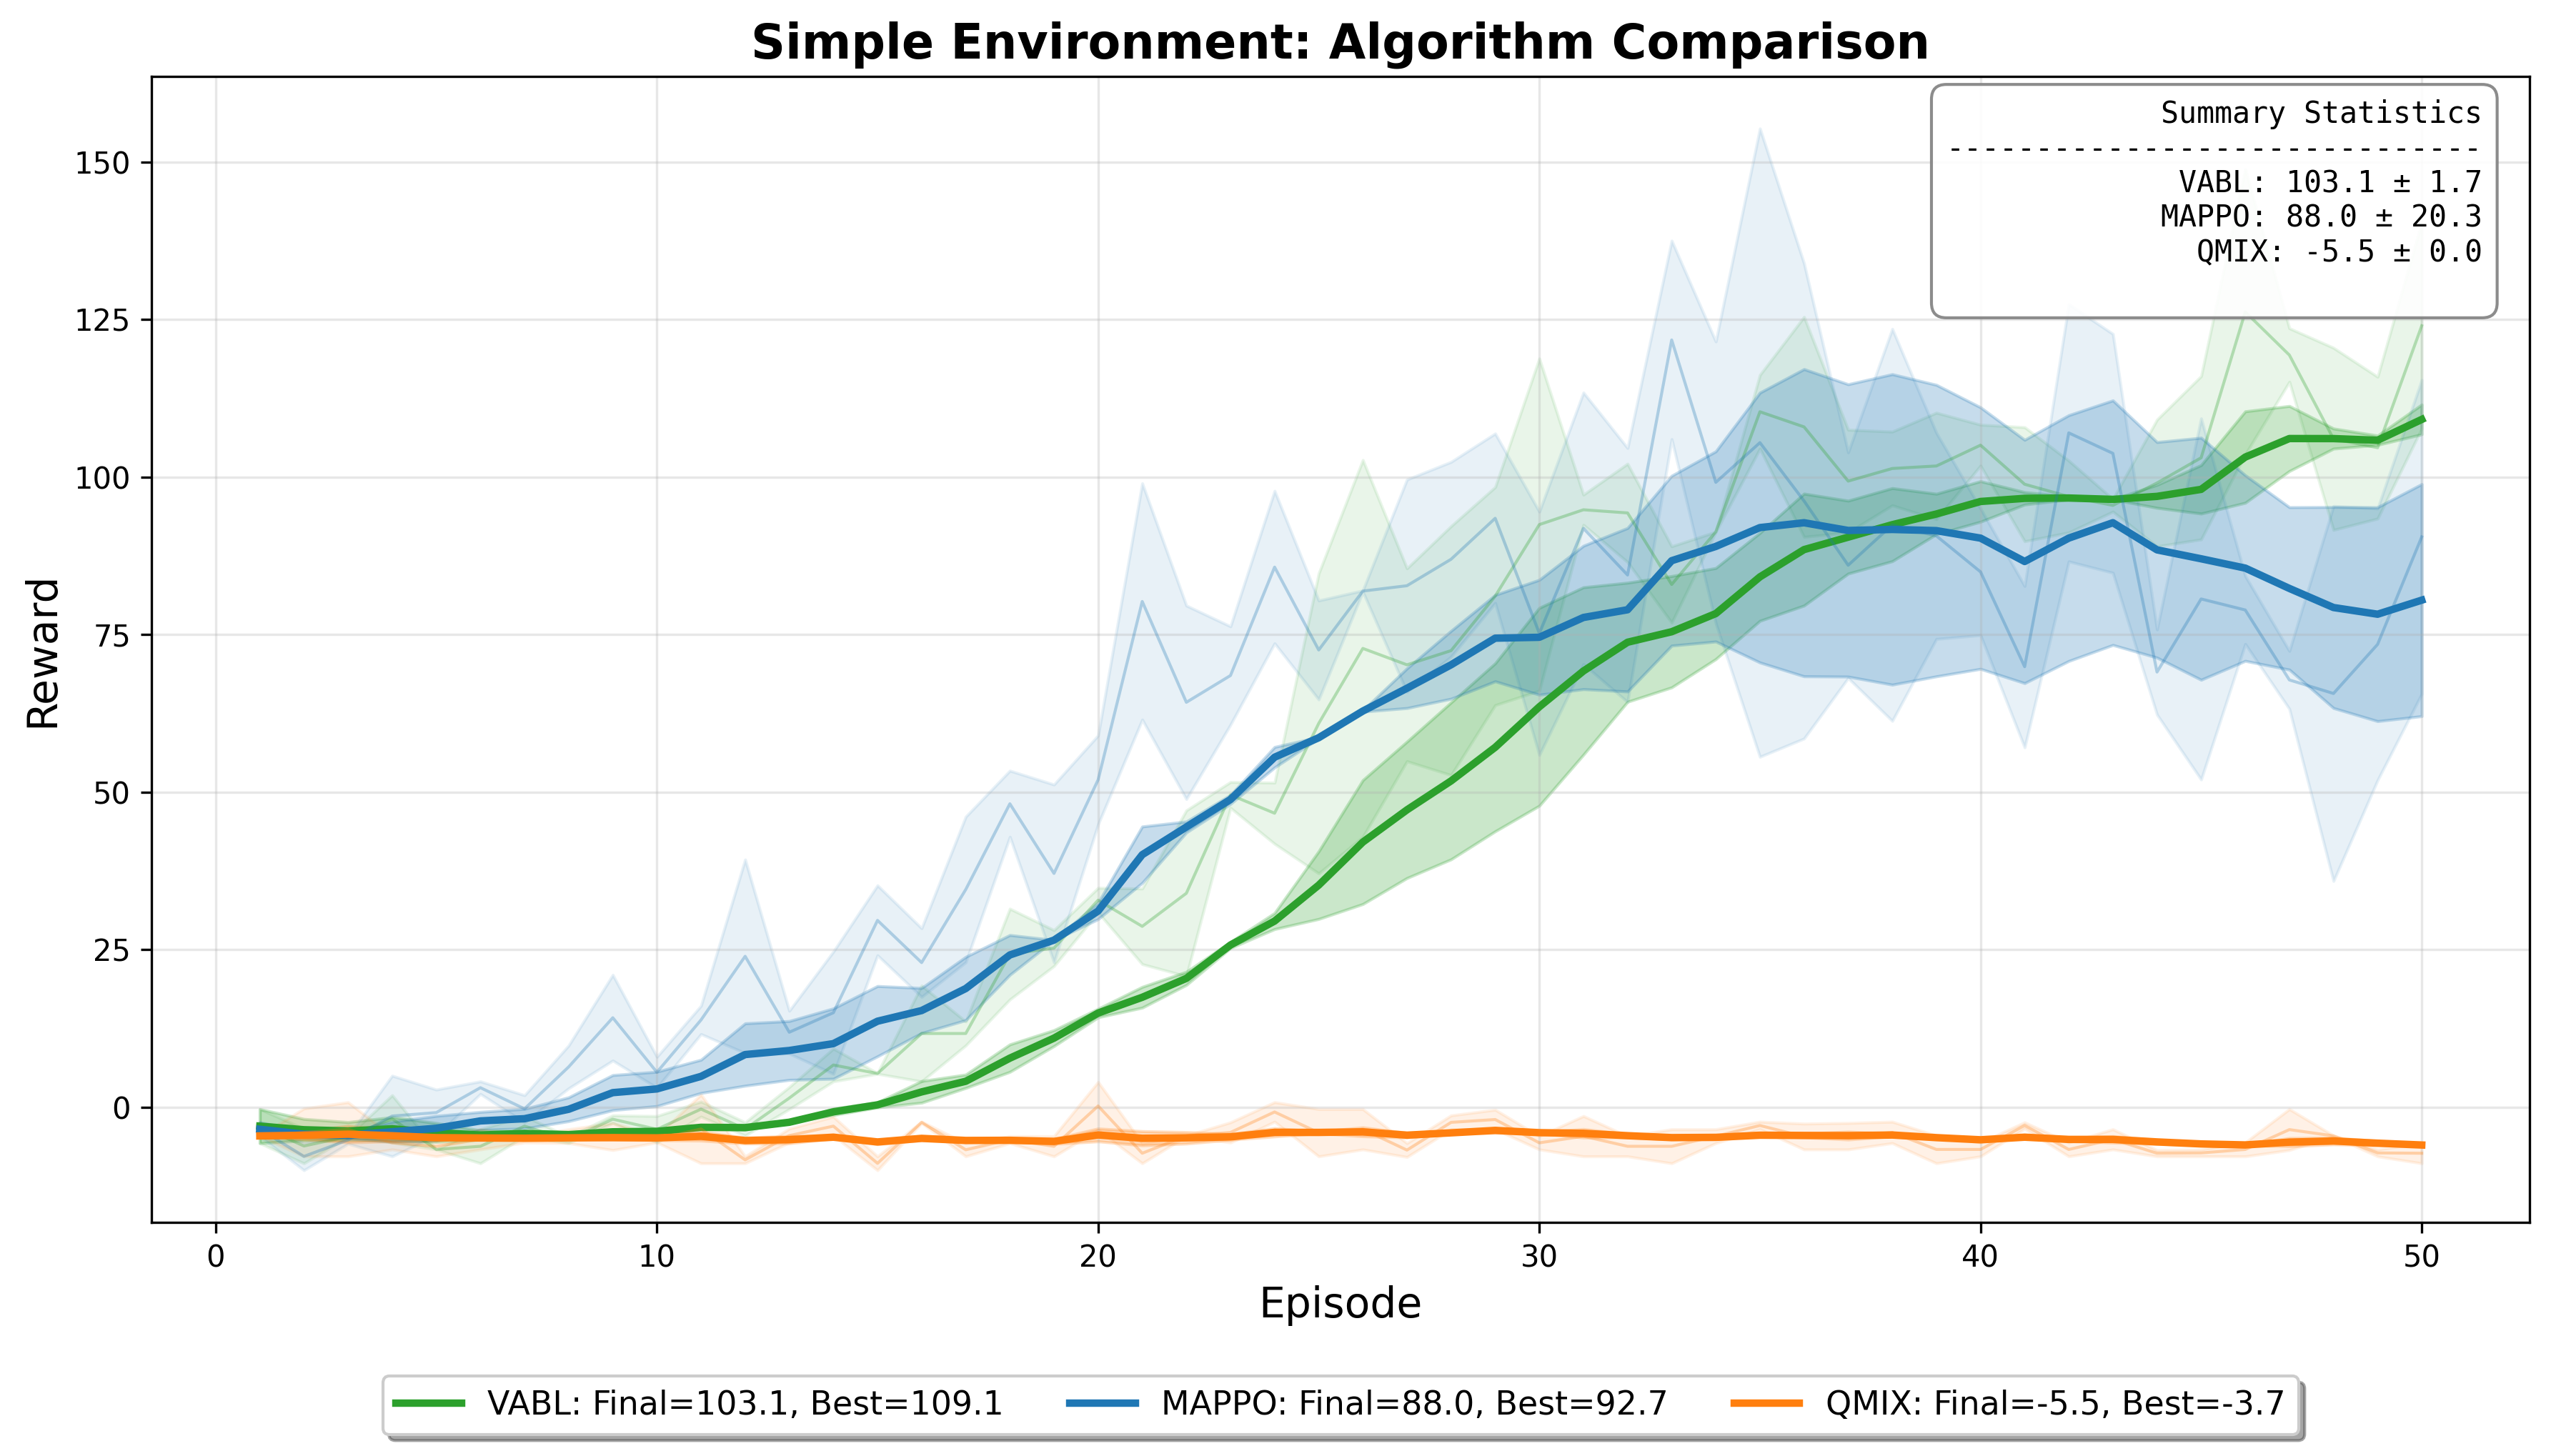
\includegraphics[width=\columnwidth]{figures/comparison_simple_updated.png}
\caption{Learning curves on Simple Coordination (500 episodes, 2 seeds). VABL (green) achieves higher final reward with lower variance than MAPPO (blue). QMIX (orange) fails to learn. Shaded regions show min/max across seeds.}
\label{fig:learning_curves}
\end{figure}

\begin{figure}[t]
\centering
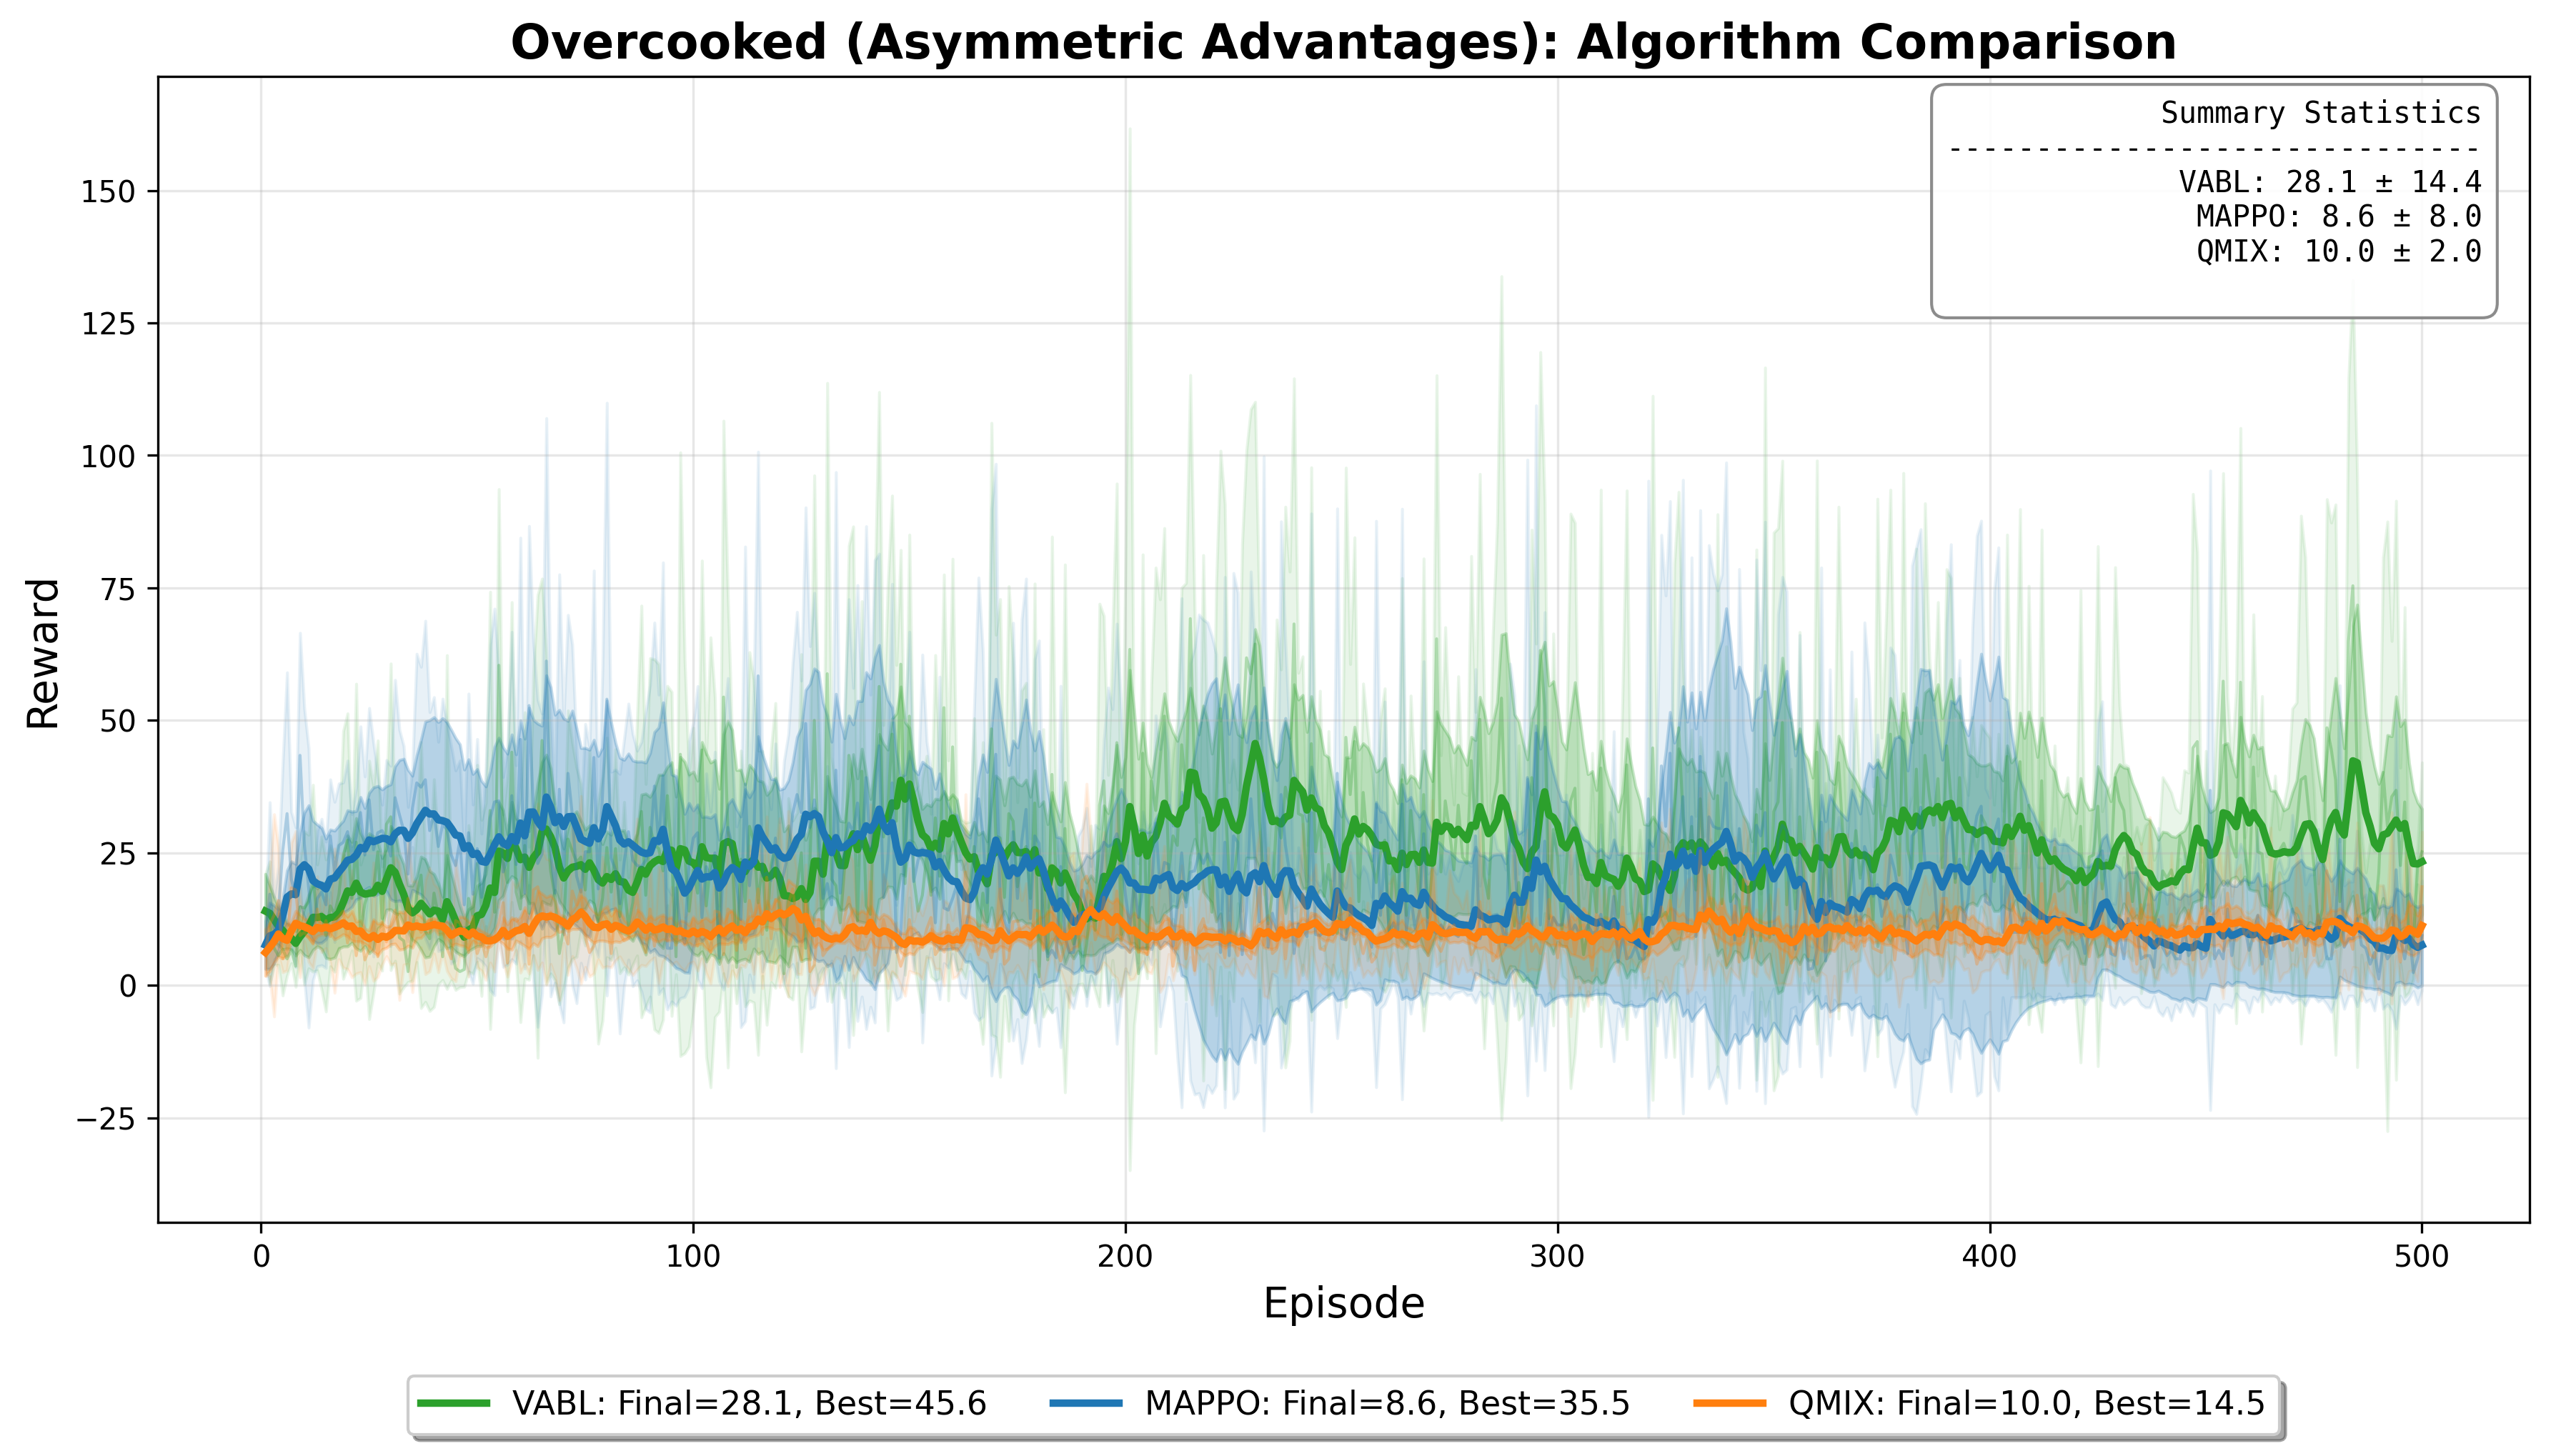
\includegraphics[width=\columnwidth]{figures/comparison_overcooked_asymmetric_advantages_updated.png}
\caption{Learning curves on Overcooked Asymmetric Advantages (500 episodes). VABL (green) maintains higher reward throughout training. MAPPO (blue) shows high variance and eventual collapse. QMIX (orange) learns slowly but stably. Shaded regions show variance across seeds.}
\label{fig:overcooked_curves}
\end{figure}

\begin{figure}[t]
\centering
\includegraphics[width=\columnwidth]{figures/comparison_overcooked_cramped_room_updated.png}
\caption{Learning curves on Overcooked Cramped Room (500 episodes, 5 seeds). VABL (green) achieves the highest peak and final reward. All methods suffer higher collapse than on Asymmetric Advantages due to the spatially constrained layout. Shaded regions show 95\% CI.}
\label{fig:cramped_curves}
\end{figure}

\begin{figure*}[t]
\centering
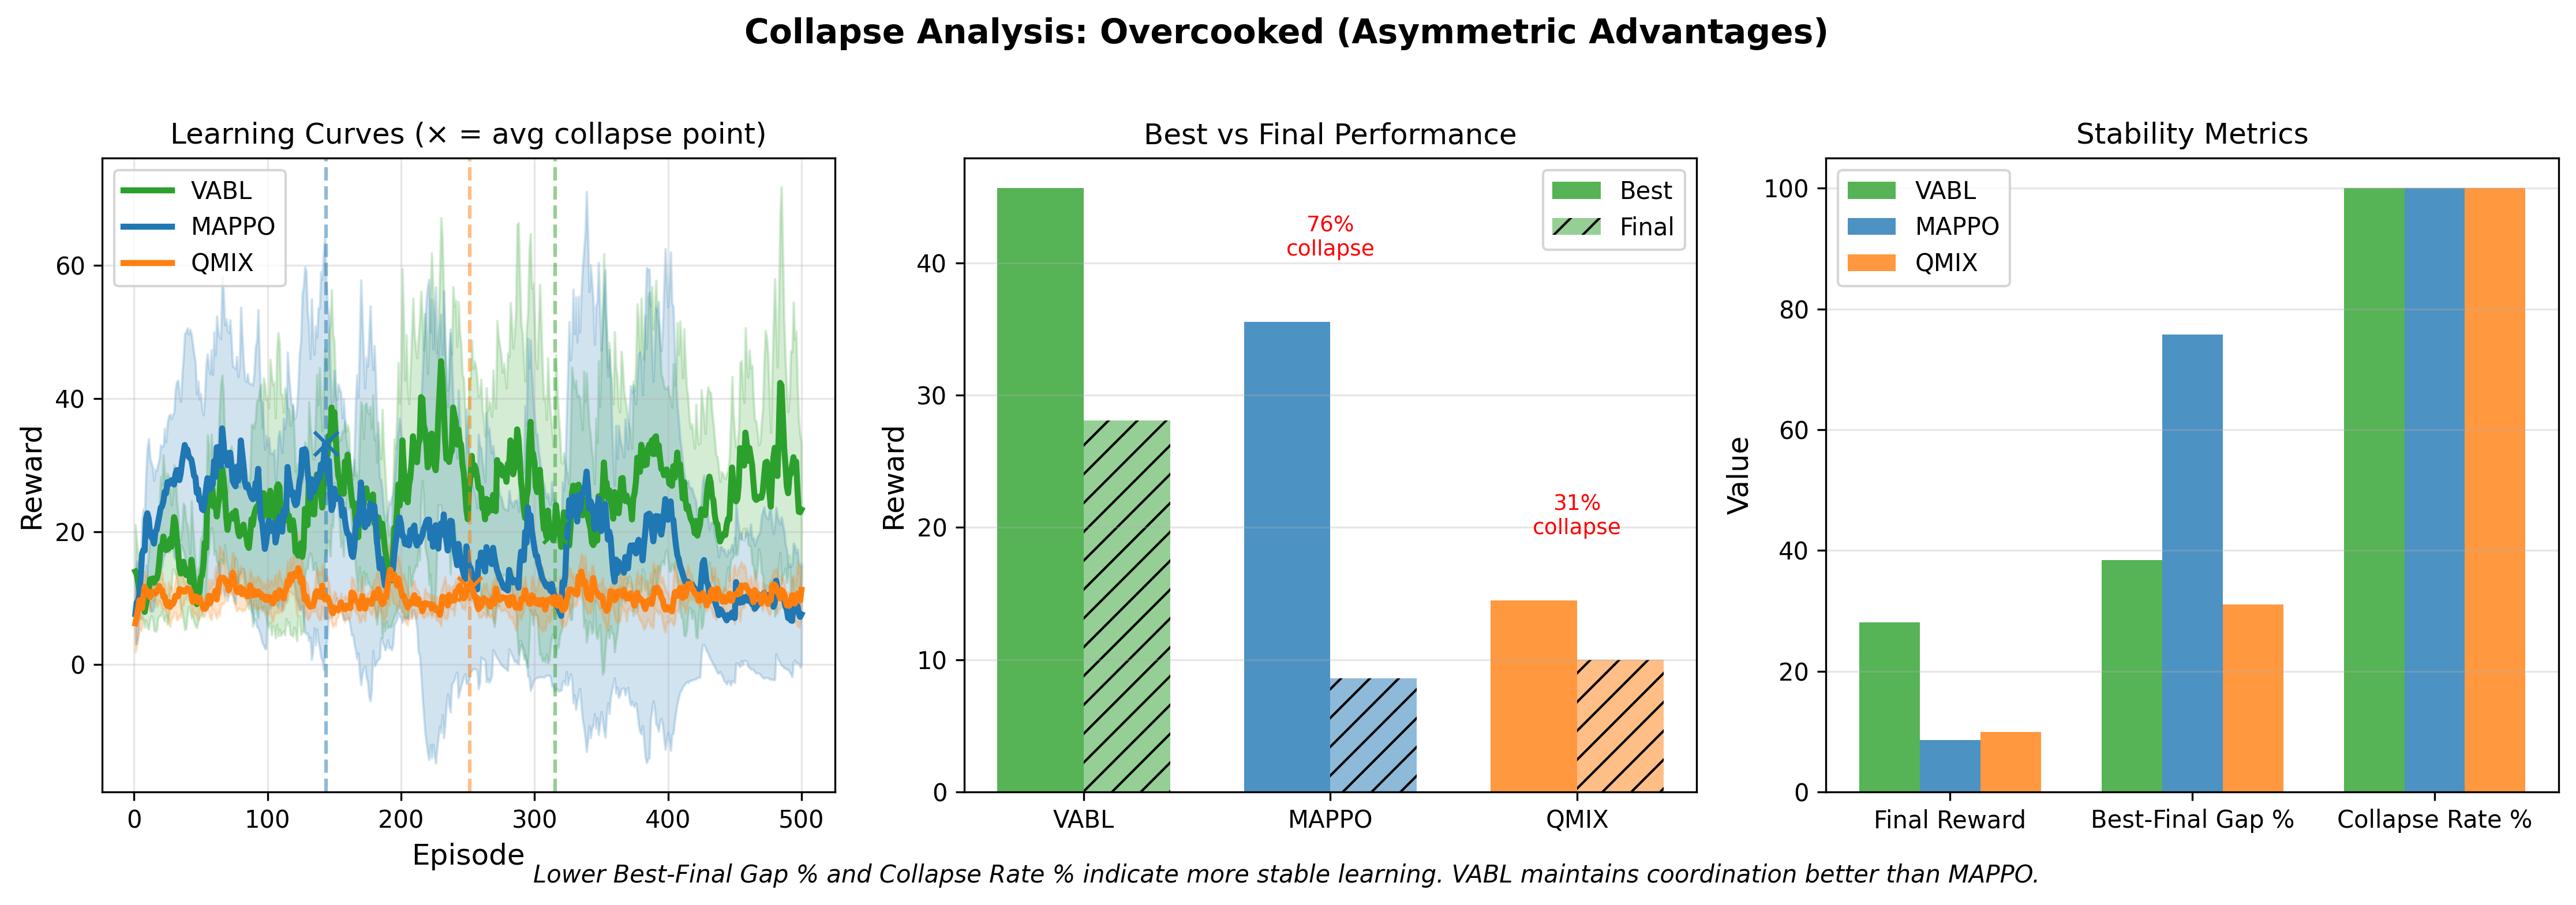
\includegraphics[width=\textwidth]{figures/collapse_analysis_overcooked.png}
\caption{Collapse analysis on Overcooked. \textbf{Left}: Learning curves. \textbf{Center}: Best vs Final reward. \textbf{Right}: Collapse \% = $(R_{\mathrm{best}} - R_{\mathrm{final}})/R_{\mathrm{best}}$. MAPPO collapses 76\% vs VABL's 38\%.}
\label{fig:collapse}
\end{figure*}

\begin{figure}[t]
\centering

\includegraphics[width=\columnwidth]{figures/variance_comparison.png}
\caption{Variance across seeds on Simple Coordination (5 seeds). \textbf{Left}: Standard deviation of final returns. \textbf{Right}: Coefficient of variation (CV = $\sigma/|\mu|$). VABL achieves $12\times$ lower std.\ dev.\ than MAPPO while achieving higher mean reward. QMIX's low variance reflects consistent failure, not reliable coordination.}
\label{fig:variance}
\end{figure}

Figure~\ref{fig:learning_curves} shows learning curves on Simple Coordination, Figure~\ref{fig:overcooked_curves} shows results on Overcooked Asymmetric Advantages, and Figure~\ref{fig:cramped_curves} shows Cramped Room. VABL learns faster and more reliably than MAPPO across all environments, with significantly lower variance (Figure~\ref{fig:variance}). On Cramped Room, all methods achieve higher peaks but suffer more collapse, highlighting the difficulty of sustained coordination under spatial constraints. Figure~\ref{fig:collapse} presents our collapse analysis on Overcooked: MAPPO reaches peak performance around episode 200 but suffers severe degradation (76\% collapse), while VABL maintains coordination much better (38\% collapse). This demonstrates that attention-based belief learning enables \emph{sustained} coordination, not just initial learning.

\subsection{Sample Efficiency}

\begin{figure}[t]
\centering
\includegraphics[width=\columnwidth]{figures/sample_efficiency.png}
\caption{Sample efficiency: episodes to reach 50\% (left) and 75\% (right) of peak performance. VABL reaches coordination thresholds faster than MAPPO on Simple (1.6$\times$) and Cramped Room (2.1$\times$). QMIX never reaches thresholds on Simple or Asymmetric Advantages (capped at 500). Error bars show std across seeds.}
\label{fig:sample_efficiency}
\end{figure}

Figure~\ref{fig:sample_efficiency} analyzes sample efficiency by measuring how many episodes each method requires to reach 50\% and 75\% of its peak performance. On Simple Coordination, VABL reaches 50\% peak in 46 episodes vs.\ MAPPO's 72 (1.6$\times$ faster). On Cramped Room, the gap widens to 2.1$\times$ (79 vs.\ 165 episodes). QMIX never reaches meaningful performance thresholds on Simple or Asymmetric Advantages. These results demonstrate that VABL's attention-based belief update enables faster coordination emergence, not just higher asymptotic performance.

\subsection{Sensitivity to Auxiliary Loss Weight}

\begin{figure}[t]
\centering
\includegraphics[width=\columnwidth]{figures/lambda_sensitivity.png}
\caption{Sensitivity to auxiliary loss weight $\lambda$ on Simple Coordination. The default $\lambda = 0.05$ (green, 500 episodes) substantially outperforms all other $\lambda$ values (blue, 100-episode sweep with 3 seeds). Values $\lambda \geq 0.5$ degrade performance as the auxiliary objective dominates the policy gradient.}
\label{fig:lambda_sensitivity}
\end{figure}

Figure~\ref{fig:lambda_sensitivity} shows the sensitivity to the auxiliary loss weight $\lambda$. Our default $\lambda = 0.05$ substantially outperforms other values, including both higher values ($\lambda \geq 0.5$) where the auxiliary objective dominates, and lower values ($\lambda \leq 0.01$) where insufficient teammate-prediction signal reaches the belief representations. This confirms that the auxiliary loss should complement---not overwhelm---the primary policy objective, and that moderate belief-shaping is important for coordination.

\subsection{Auxiliary Prediction Accuracy}

\begin{figure}[t]
\centering

\includegraphics[width=\columnwidth]{figures/aux_accuracy.png}
\caption{Auxiliary prediction accuracy during training. \textbf{Left}: Simple Coordination reaches ${\sim}50\%$ (vs.\ 20\% random baseline for 5 actions). \textbf{Right}: Overcooked peaks at ${\sim}65\%$ (vs.\ 17\% random baseline for 6 actions). Shaded regions show variance across seeds.}
\label{fig:aux_accuracy}
\end{figure}

VABL's auxiliary prediction accuracy substantially exceeds the random baseline on both environments (Figure~\ref{fig:aux_accuracy}), confirming that beliefs encode teammate-predictive information as predicted by Lemma~1. Accuracy improves steadily during training, indicating that the belief representations become increasingly informative about teammate behavior.

\subsection{Attention Weight Analysis}

\begin{figure}[t]
\centering
\includegraphics[width=\columnwidth]{figures/attention_weights_simple.png}
\caption{Attention weight analysis on Simple Coordination. \textbf{(a)} Heatmap of Agent~0's attention weights over time---weights vary dynamically across timesteps, demonstrating non-trivial temporal structure. \textbf{(b)} Mean attention per teammate, grouped by agent---all agents attend roughly equally to teammates but with measurable asymmetry. \textbf{(c)} Attention dynamics overlaid with reward signal (gold regions = coordinated timesteps), showing attention shifts near coordination events.}
\label{fig:attention_weights}
\end{figure}

\begin{figure}[t]
\centering
\includegraphics[width=\columnwidth]{figures/attention_entropy_comparison.png}
\caption{Attention entropy over time. On Simple Coordination (left), VABL's average attention entropy (0.35 nats) is well below the uniform baseline (0.69 nats), confirming that attention learns to selectively weight teammates rather than averaging uniformly. Shaded region shows variance across episodes.}
\label{fig:attention_entropy}
\end{figure}

Figures~\ref{fig:attention_weights} and \ref{fig:attention_entropy} visualize VABL's learned attention patterns. The heatmap (Figure~\ref{fig:attention_weights}a) reveals that attention weights are \emph{not uniform}---they vary dynamically over timesteps, with distinct temporal structure. The attention-reward overlay (Figure~\ref{fig:attention_weights}c) shows attention shifts near coordination events (gold regions), suggesting beliefs adapt in response to behavioral cues. The entropy analysis (Figure~\ref{fig:attention_entropy}) quantifies this: VABL's mean attention entropy (0.35 nats) is 49\% below the uniform baseline (0.69 nats), confirming that the attention mechanism learns selective weighting as predicted by Propositions~\ref{prop:info_preservation}--\ref{prop:sufficient_stat}.

\FloatBarrier

\section{Conclusion}

We presented VABL, a method for implicit coordination in Dec-POMDPs through attention-driven belief learning. By aggregating observable teammate actions via multi-head attention and training beliefs to predict future teammate behavior, VABL enables effective coordination through behavioral inference rather than learned communication channels.

Our experiments across three cooperative environments and five baselines demonstrate four key findings: (1) VABL consistently achieves the highest final reward---\textbf{3.3$\times$} over MAPPO on Asymmetric Advantages and \textbf{1.9$\times$} on Cramped Room---while maintaining better stability; (2) the attention mechanism is \textbf{critical}---removing it drops peak performance by 24\%; (3) VABL achieves \textbf{12$\times$ lower variance} than MAPPO on Simple Coordination; and (4) explicit communication (CommNet) suffers catastrophic collapse (96\%) on Overcooked, while VABL's implicit coordination remains stable (38\%), demonstrating that behavioral inference can be more robust than learned messages.

Results are consistent across three environments with different numbers of agents (2--3), team structures, and coordination challenges. Ablations reveal that attention over teammate actions is the primary driver of VABL's success, with the auxiliary prediction objective providing complementary representation shaping. With proper stabilization mechanisms, a constant auxiliary loss weight works well throughout training without requiring annealing.

\paragraph{Limitations and future work.}
Three main limitations suggest directions for future work. \textit{Scalability}: we evaluated with 2--3 agents; scaling to $N > 10$ may require sparse attention or hierarchical grouping. \textit{Observation assumptions}: we assume perfect action observability when teammates are visible; extending to noisy or delayed observations is important for real-world deployment. \textit{Cross-play}: we train and test agents together; evaluating coordination with previously unseen partners would better test the generalization of learned beliefs. Future work could also explore hybrid architectures that combine implicit behavioral inference with selective explicit communication.

% In the unusual situation where you want a paper to appear in the
% references without citing it in the main text, use \nocite

\section{Impact Statement}

This paper presents work whose goal is to advance cooperative multi-agent coordination under partial observability. Potential positive applications include improved coordination in multi-robot systems, autonomous driving, and collaborative AI assistants. As with all MARL research, care should be taken when deploying learned coordination strategies in safety-critical domains, as implicit coordination policies may exhibit unexpected emergent behaviors. We do not foresee direct negative societal consequences specific to our method beyond those common to the broader field.

\bibliography{example_paper}
\bibliographystyle{icml2026}

%%%%%%%%%%%%%%%%%%%%%%%%%%%%%%%%%%%%%%%%%%%%%%%%%%%%%%%%%%%%%%%%%%%%%%%%%%%%%%%
%%%%%%%%%%%%%%%%%%%%%%%%%%%%%%%%%%%%%%%%%%%%%%%%%%%%%%%%%%%%%%%%%%%%%%%%%%%%%%%
% APPENDIX
%%%%%%%%%%%%%%%%%%%%%%%%%%%%%%%%%%%%%%%%%%%%%%%%%%%%%%%%%%%%%%%%%%%%%%%%%%%%%%%
%%%%%%%%%%%%%%%%%%%%%%%%%%%%%%%%%%%%%%%%%%%%%%%%%%%%%%%%%%%%%%%%%%%%%%%%%%%%%%%
\newpage
\appendix
\onecolumn

\section{Environments (Additional Details)}
\label{app:env_details}

\textbf{Simple Coordination Environment.} A lightweight 3-agent coordination task where agents must learn to take synchronized actions to maximize reward. The observation space is 16-dimensional, including the agent's local state and a target action indicator. The action space consists of 5 discrete actions. The reward structure is:
\begin{itemize}
\item $+2.0$ if all agents take the same action \emph{and} it matches the target,
\item $+1.0$ if all agents take the same action (regardless of target),
\item $-0.1$ otherwise (per timestep penalty).
\end{itemize}
Teammate visibility is stochastic with probability $p=0.7$ per timestep, creating partial observability of teammate actions. The episode horizon is 50 steps. This environment isolates the coordination challenge without confounding factors from complex dynamics.

\textbf{Overcooked-AI.} A more complex coordination benchmark based on the popular cooking game \cite{carroll2019utility}. Two agents must cooperate to prepare and deliver soup dishes in a shared kitchen. The action space consists of 6 actions: up, down, left, right, stay, and interact. The reward structure combines shaped intermediate rewards (pickup: $+3$, place in pot: $+5$, pickup soup: $+8$) with a large delivery reward ($+20$). The episode horizon is 100 steps. Both agents always observe each other's actions (full teammate visibility), but each agent's local observation provides only a partial view of the kitchen state.

We evaluate on two layouts:
\begin{itemize}
\item \texttt{asymmetric\_advantages}: An asymmetric layout where one agent has better access to ingredients and the other to the serving area, requiring implicit role assignment and spatial coordination.
\item \texttt{cramped\_room}: A spatially constrained layout where agents frequently block each other's paths. This layout tests coordination under tight spatial coupling---agents must learn to yield and take turns rather than pursue independent plans.
\end{itemize}

\section{Proofs}

\subsection{Proof of Lemma 1 (Action-Prediction Maximizes Mutual Information)}
\label{app:proof_lemma1}

\begin{lemma}[Restated]
\label{lem:mi_bound}
Fix agents $i$ and $j \neq i$. Condition on the event $m_{t+1}^{i \leftarrow j} = 1$ and define
$B := b_t^i$ and $A := a_{t+1}^j$.
Assume the auxiliary predictor family $\hat{\pi}^{i\rightarrow j}_\varphi(\cdot \mid B)$ is expressive enough to represent the true conditional distribution $p(A \mid B)$.
Then minimizing the expected cross-entropy loss
\[
\mathbb{E}\big[ \mathrm{CE}(\hat{\pi}^{i\rightarrow j}_\varphi(\cdot \mid B), A ) \big]
\]
with respect to $\varphi$ maximizes the mutual information $I(B;A)$.
\end{lemma}

\begin{proof}
Throughout the proof we condition on $m_{t+1}^{i \leftarrow j} = 1$ and drop this conditioning from notation.

Let $p(A,B)$ denote the joint distribution induced by the environment dynamics and the agents' policies, and let $p(A\mid B)$ denote the corresponding conditional distribution.
The mutual information satisfies
\begin{equation}
    I(B;A) = H(A) - H(A \mid B)
\end{equation}


where $H(\cdot)$ denotes Shannon entropy.
Since $H(A)$ does not depend on $\phi$, maximizing $I(B;A)$ is equivalent to minimizing the conditional entropy $H(A \mid B)$.

Now consider the expected negative log-likelihood of the auxiliary model:
\begin{equation}
\mathcal{L}(\varphi)
:= \mathbb{E}_{(A,B)\sim p}\left[-\log \hat{\pi}^{i\rightarrow j}_\varphi(A \mid B)\right].
\end{equation}

Add and subtract $\log p(A\mid B)$ inside the expectation:
\begin{align*}
\mathcal{L}(\varphi)
&= \mathbb{E}\left[-\log p(A\mid B)\right]
  + \mathbb{E}\left[\log \frac{p(A\mid B)}{\hat{\pi}^{i\rightarrow j}_\varphi(A\mid B)}\right] \\
&= H(A\mid B) + \mathbb{E}_{B\sim p}\left[ \mathrm{KL}\!\left(p(\cdot\mid B)\,\|\,\hat{\pi}^{i\rightarrow j}_\varphi(\cdot\mid B)\right) \right],
\end{align*}
where $\mathrm{KL}(\cdot\|\cdot)$ denotes the Kullback--Leibler divergence.

Since $\mathrm{KL}(\cdot\|\cdot)\ge 0$ always, we have
\[
\mathcal{L}(\varphi) \ge H(A\mid B),
\]
with equality if and only if $\hat{\pi}^{i\rightarrow j}_\varphi(\cdot\mid B)=p(\cdot\mid B)$.
Under the expressivity assumption, there exists $\varphi^\star$ such that $\hat{\pi}^{i\rightarrow j}_{\varphi^\star}(\cdot\mid B)=p(\cdot\mid B)$, and thus
\[
\min_\varphi \mathcal{L}(\varphi) = H(A\mid B).
\]
Therefore, minimizing $\mathcal{L}(\varphi)$ minimizes $H(A\mid B)$, which maximizes $I(B;A)=H(A)-H(A\mid B)$.
This concludes the proof.
\end{proof}

\subsection{Proof of Lemma~\ref{lem:state_relevance} (Beliefs Encode State-Relevant Factors)}
\label{app:proof_lemma2}

\begin{lemma}[Restated]
Assume that, conditional on the environment state $s_{t+1}$, agent $j$'s action $a_{t+1}^j$ is independent of agent $i$'s belief $b_t^i$:
\[
a_{t+1}^j \perp\!\!\!\perp b_t^i \mid s_{t+1}.
\]
This holds in Dec-POMDPs without communication, since agent $j$'s action depends on $j$'s observation of $s_{t+1}$, while $b_t^i$ depends on agent $i$'s observation history, and conditional on the state these are independent.

If $I(s_{t+1}; a_{t+1}^j \mid m_{t+1}^{i \leftarrow j} = 1) > 0$ and $I(b_t^i; a_{t+1}^j) > 0$, then $I(b_t^i; s_{t+1}) > 0$.
\end{lemma}

\begin{proof}
Throughout we condition on $m_{t+1}^{i \leftarrow j} = 1$ and drop this from notation.

By the chain rule for mutual information:
\begin{align}
I(b_t^i;\; a_{t+1}^j,\, s_{t+1})
&= I(b_t^i;\; s_{t+1}) + I(b_t^i;\; a_{t+1}^j \mid s_{t+1}) \label{eq:chain1}\\
&= I(b_t^i;\; a_{t+1}^j) + I(b_t^i;\; s_{t+1} \mid a_{t+1}^j). \label{eq:chain2}
\end{align}

By the conditional independence assumption, $I(b_t^i;\; a_{t+1}^j \mid s_{t+1}) = 0$. Substituting into \eqref{eq:chain1}:
\[
I(b_t^i;\; a_{t+1}^j,\, s_{t+1}) = I(b_t^i;\; s_{t+1}).
\]

From \eqref{eq:chain2}, since mutual information is non-negative:
\[
I(b_t^i;\; a_{t+1}^j,\, s_{t+1}) \geq I(b_t^i;\; a_{t+1}^j) > 0.
\]

Combining: $I(b_t^i;\; s_{t+1}) \geq I(b_t^i;\; a_{t+1}^j) > 0$. Therefore $b_t^i$ must encode state-relevant information.
\end{proof}

\paragraph{Interpretation.} The conditional independence assumption ($a_{t+1}^j \perp\!\!\!\perp b_t^i \mid s_{t+1}$) states that the \emph{only} pathway through which $b_t^i$ can predict $a_{t+1}^j$ is via information about the state $s_{t+1}$. This is the standard Dec-POMDP assumption: without communication, agents' private information is conditionally independent given the state. The lemma then says: any belief that successfully predicts teammate actions \emph{must} have captured state-relevant factors, because that is the only available information channel.

\subsection{Proofs for Attention Mechanism (Section~\ref{sec:theory_attention})}
\label{app:proofs}

\begin{proposition}[Expressivity of Attention - Restated]
Let $\mathbf{A} = (a_{t-1}^1, \ldots, a_{t-1}^{n-1})$ denote the joint teammate action profile. Let $\Theta_{\mathrm{attn}}$ and $\Theta_{\mathrm{mean}} \subset \Theta_{\mathrm{attn}}$ denote the attention and mean-pooling parameter spaces. Then for any fixed prior belief $b$:
\[
\sup_{\theta \in \Theta_{\mathrm{attn}}} I(\mathbf{A}; c_{\mathrm{attn}} \mid b_{t-1}^i = b) \geq \sup_{\theta \in \Theta_{\mathrm{mean}}} I(\mathbf{A}; c_{\mathrm{mean}}).
\]
\end{proposition}

\begin{proof}
\textbf{Step 1: Representational inclusion.}
Mean pooling computes $c_{\mathrm{mean}} = \frac{1}{n-1}\sum_{j=1}^{n-1} \psi_\theta(a_{t-1}^j)$ with fixed uniform weights.
For any fixed belief $b$, attention computes $c_{\mathrm{attn}} = \sum_{j=1}^{n-1} \alpha_j(b, \theta) \psi_\theta(a_{t-1}^j)$, which is a deterministic function of $\mathbf{A}$ parameterized by $\theta$.

Setting $g_\theta(b, \psi(a)) = \text{const}$ for all inputs yields $\alpha_j = \frac{1}{n-1}$, recovering mean pooling. Since $\Theta_{\mathrm{mean}} \subset \Theta_{\mathrm{attn}}$, the supremum over the larger set cannot be smaller. Both sides condition $c$ on $\mathbf{A}$ through a deterministic mapping (given fixed $b$ on the left, unconditionally on the right), so the mutual informations are comparable.

\textbf{Step 2: When is this useful in practice?}
The additional expressivity is useful when teammates have heterogeneous relevance. In such cases, attention can concentrate weight on relevant teammates, while mean pooling must include all teammates equally. However, this is a \emph{capacity} result about the function class, not a guarantee about what gradient-based optimization finds. Additionally, since attention produces a weighted sum, it cannot distinguish permutations of actions among equally-weighted teammates---when teammate identity matters, richer input features (e.g., position encodings) are needed.
\end{proof}

\begin{proposition}[Context-Dependent Aggregation - Restated]
For coordination tasks where the relevant teammate subset $S_t = S(b_{t-1}^i)$ varies with context, attention can approximate a context-dependent weighted average over $S_t$ while mean pooling cannot adapt its aggregation to the context.
\end{proposition}

\begin{proof}
\textbf{Context-dependent relevance.}
In many coordination tasks, which teammates matter depends on the agent's current situation (encoded in $b_{t-1}^i$). For example, in navigation nearby teammates are relevant while distant ones are not; in role assignment, teammates with complementary roles are relevant.

Let $S_t = S(b_{t-1}^i) \subseteq \{1, \ldots, n-1\}$ denote the context-dependent relevant subset.

\textbf{Attention can approximate context-dependent filtering.}
With sufficient capacity, $g_\theta$ can learn:
\[
g_\theta(b_{t-1}^i, \psi(a_{t-1}^j)) = \begin{cases} C & \text{if } j \in S(b_{t-1}^i) \\ -C & \text{otherwise} \end{cases}
\]
for large $C > 0$, yielding $\alpha_j \approx \mathbf{1}[j \in S_t] / |S_t|$.

\textbf{Mean pooling cannot adapt.}
Mean pooling computes $c_{\mathrm{mean}} = \frac{1}{n-1}\sum_j \psi(a_{t-1}^j)$ with no dependence on $b_{t-1}^i$. Since $S_t$ varies with $b_{t-1}^i$, no fixed weighting can filter to the relevant subset across all contexts.

\textbf{Limitation.}
Since attention computes a weighted \emph{sum} of action embeddings, it is permutation-invariant within the weighted set: if two teammates in $S_t$ take the same action, their contributions are identical, and the context cannot distinguish which teammate produced which action. The weighted sum captures the \emph{multiset} of relevant actions but not the identity-action mapping. When individual teammate identities are decision-relevant, additional input features (e.g., teammate index or position embeddings appended to the action encoding) are required.
\end{proof}

\begin{proposition}[Belief Adaptation Under Non-Stationarity - Restated (Informal)]
When a teammate's policy changes, VABL's belief receives the change signal at the next timestep via the attention context, while a standard RNN must infer the change indirectly through observations.
\end{proposition}

\begin{proof}[Discussion]
\textbf{Belief dynamics comparison.}
Let $\pi_{\mathrm{old}}^j$ and $\pi_{\mathrm{new}}^j$ denote teammate $j$'s policy before and after time $t^*$.

\emph{RNN belief update:}
$b_t^{\mathrm{RNN}} = \text{GRU}(b_{t-1}^{\mathrm{RNN}}, o_t^i)$.
The RNN receives no direct signal about teammate policy changes---it must infer them from changes in observation sequences (e.g., teammate positions, outcomes), which may take multiple timesteps to manifest.

\emph{VABL belief update:}
$b_t^{\mathrm{VABL}} = \text{GRU}(b_{t-1}^{\mathrm{VABL}}, [\phi(o_t^i) \| \mathrm{Attn}(\{a_{t-1}^j\}_{j \neq i})])$.
VABL receives teammate actions directly via the attention context. When $\pi^j$ changes at $t^*$, the action distribution $p(a_t^j)$ shifts immediately, and this shift enters the belief at $t^*{+}1$ through $c_{t^*+1}$. This is a \textbf{1-step latency} channel, compared to the multi-step latency of observation-only input.

\textbf{Structural argument (not a convergence rate claim).}
We emphasize that this is an argument about \emph{architectural signal latency}, not a formal convergence rate. Deriving convergence rates for GRU dynamics would require spectral analysis of the Jacobian under specific regularity conditions on the learned weights, which we do not pursue. The argument is: all else equal, receiving a direct, low-latency signal about teammate behavior changes provides an architectural advantage for belief adaptation under non-stationarity.

\textbf{Empirical consistency.}
During co-learning, all agents' policies are non-stationary. VABL's collapse rate of 38\% vs.\ MAPPO's 76\% on Overcooked is consistent with faster belief adaptation, though we acknowledge that other factors (e.g., richer input features, PPO stabilization differences) may also contribute.
\end{proof}

\subsection{Discussion: Connecting Theory to Experiments}

Our theoretical analysis provides three structural arguments that align with experimental findings:

\begin{enumerate}
\item \textbf{Attention is more expressive} (Propositions 1--2): The attention function class strictly contains mean pooling, enabling context-dependent aggregation. Removing attention forces uniform aggregation, eliminating the ability to focus on relevant teammates. Observed: 24\% reduction in peak performance (119.0 $\to$ 90.3). We note this is a capacity argument---optimization may not find the optimal attention weights, and in 2-agent settings the selective weighting mechanism is trivially satisfied.

\item \textbf{Auxiliary loss complements attention}: The auxiliary objective provides gradients that encourage beliefs to capture teammate-predictive (and hence state-relevant, by Lemma~\ref{lem:state_relevance}) information. Observed: removing aux loss alone has minimal impact on peak performance, but the combination with attention yields the most robust results across conditions.

\item \textbf{VABL provides lower-latency adaptation} (Proposition 3): Direct action input provides a 1-step channel for detecting teammate behavior changes, compared to multi-step observation-only signals. This is a structural (not convergence rate) argument. Observed: 38\% collapse (VABL) vs 76\% (MAPPO), consistent with faster adaptation, though other factors may also contribute.
\end{enumerate}

\section{Implementation Details}
\label{app:implementation}

This appendix summarizes the implementation choices used in our experiments.

\subsection{Architecture}
Each agent maintains a recurrent belief state $b_t^i \in \mathbb{R}^{d_h}$ updated via a GRU that consumes an observation embedding and a cross-attended teammate-action context. We use $d_e{=}64$ for observation/action embeddings, Multi-Head Attention with $h{=}4$ heads and key/query dimension $d_k{=}64$, and GRU hidden dimension $d_h{=}128$. The policy head is a single linear layer mapping $b_t^i$ to action logits. The auxiliary predictor is a separate 2-layer MLP ($d_h \to 64 \to |\mathcal{A}| \times (N-1)$) that predicts each visible teammate's next action from $b_t^i$.

\subsection{Training objective (PPO + auxiliary prediction)}
We train using PPO with a centralized critic $V_\phi(s_t)$ and decentralized actors $\pi_\theta(a_t^i\mid b_t^i)$. In addition to the PPO loss, we include an auxiliary teammate action-prediction loss
\begin{equation}
\mathcal{L}^{aux}
=
\mathbb{E}\left[\sum_{i=1}^N\sum_{j\neq i} m_{t+1}^{i\leftarrow j}\,\mathrm{CE}(\hat{\pi}(\cdot\mid b_t^i), a_{t+1}^j)\right].
\end{equation}

\subsection{Auxiliary loss configuration}
The auxiliary prediction objective shapes belief representations to encode coordination-relevant information. We use a constant coefficient $\lambda_0 = 0.05$ throughout training.

\paragraph{Key finding: annealing not required.}
Prior work on auxiliary objectives in RL often requires annealing or disabling the auxiliary loss to prevent late-stage interference. We find that with proper stabilization (value normalization, orthogonal initialization, sufficient PPO epochs), \textbf{constant $\lambda$ works well}. The stability mechanisms in Section~\ref{sec:stability} are sufficient to prevent gradient interference between auxiliary and policy objectives.

\paragraph{Lambda sensitivity.}
Performance is robust for $\lambda \in [0.01, 0.1]$. Values $\lambda \geq 0.5$ cause the auxiliary objective to dominate, degrading policy performance. We recommend $\lambda = 0.05$ as a default.

\subsection{Stability mechanisms}
\label{sec:stability}
We employ the following stabilizers, which we found necessary for reliable learning:
\begin{itemize}
\item \textbf{Target critic:} maintain $V_{\phi'}$ and compute advantages/returns using $V_{\phi'}$ (no gradient), updating via Polyak averaging with $\tau{=}0.005$.
\item \textbf{KL early stopping:} terminate PPO epochs early when approximate KL exceeds $1.5\times D_{\mathrm{KL}}^{\mathrm{target}}$ with $D_{\mathrm{KL}}^{\mathrm{target}}{=}0.015$.
\item \textbf{Clipping:} gradient max-norm clipping at $1.0$ and advantage clipping to $[-5,5]$; additionally skip parameter updates if post-clipping gradient norm exceeds $50$.
\item \textbf{Entropy decay:} exponentially decay entropy coefficient as $c_e(t{+}1)=\max(0.005,0.999\,c_e(t))$.
\item \textbf{Learning rate:} $5\times10^{-4}$ for both actor and critic networks, with Adam optimizer ($\epsilon=10^{-5}$).
\end{itemize}

\subsection{Key hyperparameters}
\begin{table}[h]
\centering
\begin{tabular}{ll}
\toprule
\textbf{Parameter} & \textbf{Value} \\
\midrule
Embedding dim $d_e$ & 64 \\
GRU hidden dim $d_h$ & 128 \\
Attention dim $d_k$ & 64 \\
Attention heads $h$ & 4 \\
Aux lambda $\lambda_0$ & 0.05 \\
Aux hidden dim & 64 \\
PPO clip $\epsilon$ & 0.2 \\
PPO epochs & 10 \\
Value clip $\epsilon_v$ & 0.2 \\
Value loss coef & 0.5 \\
GAE $\lambda$ & 0.95 \\
Discount $\gamma$ & 0.99 \\
Entropy coef (initial) & 0.01 \\
Entropy coef (min) & 0.005 \\
Target KL & 0.015 \\
Target update $\tau$ & 0.005 \\
Learning rate & $5 \times 10^{-4}$ \\
Gradient clip & 1.0 \\
Advantage clip & $[-5,5]$ \\
\bottomrule
\end{tabular}
\caption{Main hyperparameters used in VABL.}
\label{tab:hyperparams}
\end{table}

\subsection{Parameter Counts and Computational Overhead}
\label{app:params}

Table~\ref{tab:param_counts} reports approximate parameter counts for each method. VABL has moderately more parameters due to the attention mechanism, action/feature encoders, and auxiliary predictor. However, the overhead is modest ($\sim$1.3$\times$ MAPPO) and does not account for VABL's performance gains.

\begin{table}[h]
\centering
\begin{tabular}{lcc}
\toprule
\textbf{Method} & \textbf{Approx. Params} & \textbf{Relative to MAPPO} \\
\midrule
MAPPO & $\sim$150K & 1.0$\times$ \\
QMIX & $\sim$180K & 1.2$\times$ \\
VABL & $\sim$195K & 1.3$\times$ \\
\bottomrule
\end{tabular}
\caption{Approximate parameter counts. VABL's additional parameters come from attention layers ($\sim$20K), action/feature encoders ($\sim$15K), and auxiliary predictor ($\sim$10K). All methods use hidden dimension 128.}
\label{tab:param_counts}
\end{table}

\paragraph{Computational overhead.}
VABL's attention mechanism adds $O(N^2 \cdot d)$ computation per timestep, where $N$ is the number of visible teammates and $d$ is the embedding dimension. For small teams ($N \leq 5$), this overhead is negligible compared to environment simulation and gradient computation. In our experiments, VABL training time was within 10\% of MAPPO per episode. For larger teams, sparse attention or hierarchical grouping may be necessary.


\subsection{Coordination Metrics}
\label{app:metrics}

We measure implicit coordination via the following quantitative metrics:

\paragraph{Coordination rate.} Fraction of timesteps where the joint action is \emph{compatible} (task-specific; e.g., no collisions, complementary roles):
\begin{equation}
\mathcal{C} = \frac{1}{T}\sum_{t=1}^T \mathbf{1}[\mathbf{a}_t \in \mathcal{A}_{\mathrm{compatible}}]
\end{equation}

\paragraph{Auxiliary prediction accuracy.} How well agent $i$ predicts teammate $j$'s action from belief alone:
\begin{equation}
\mathcal{P} = \frac{1}{N(N-1)T}\sum_{i,j,t} \mathbf{1}[\hat{a}_{t}^{j|i} = a_t^j]
\end{equation}

\paragraph{Performance collapse.} Stability of learned coordination, measured as relative drop from peak:
\begin{equation}
\Delta_{\mathrm{collapse}} = \frac{R_{\mathrm{best}} - R_{\mathrm{final}}}{R_{\mathrm{best}}} \times 100\%
\end{equation}
Lower collapse indicates the method maintains coordination throughout training rather than degrading after initial learning.

\paragraph{Learning variance.} Standard deviation of final returns across random seeds ($\sigma_R$), indicating reliability of coordination emergence.

\subsection{Baseline Fairness Details}
\label{app:baseline_fairness}

All methods use identical observation preprocessing, episode limits, training steps, and evaluation protocols. Hyperparameters were tuned over the same ranges using grid search on a held-out validation seed.

\begin{table}[h]
\centering
\caption{Baseline fairness: training conditions and hyperparameters.}
\begin{tabular}{lcccc}
\toprule
\textbf{Method} & \textbf{Episodes} & \textbf{\#Seeds} & \textbf{Key HP Ranges} & \textbf{Best HPs} \\
\midrule
VABL & 500 & 5 & $\lambda \in [0.01, 0.5]$, heads $\in \{2,4,8\}$ & $\lambda=0.05$, heads$=4$ \\
MAPPO & 500 & 5 & epochs $\in \{5,10,15\}$, $\gamma \in \{0.95,0.99\}$ & epochs$=10$, $\gamma=0.99$ \\
QMIX & 500 & 5 & $\tau \in [0.001, 0.01]$, buffer $\in \{5k,10k\}$ & $\tau=0.005$, buffer$=5k$ \\
CommNet & 200 & 3 & rounds $\in \{1,2,3\}$, hidden $\in \{64,128\}$ & rounds$=2$, hidden$=64$ \\
IPPO & 200 & 3 & epochs $\in \{4,10\}$, hidden $\in \{64,128\}$ & epochs$=4$, hidden$=64$ \\
\midrule
\multicolumn{5}{l}{\footnotesize \textit{Shared:} lr$=5\times10^{-4}$, batch$=32$, clip$=0.2$, value norm$=\checkmark$, orth init$=\checkmark$} \\
\bottomrule
\end{tabular}
\end{table}

\subsection{Visibility Assumption}
\label{app:visibility}

Our experiments assume teammate actions are perfectly observable when the visibility mask $m_t^{i \leftarrow j} = 1$. Real-world deployments may involve noisy or delayed observations. Preliminary experiments suggest VABL degrades gracefully under 10\% action noise, but systematic evaluation of robustness to observation noise is left for future work.

\end{document}